\documentclass[a4paper]{article}

\input{style/ch_xelatex.tex}
\input{style/scala.tex}

\usepackage{titlesec}
\titleclass{\subsubsubsection}{straight}[\subsection]

\newcounter{subsubsubsection}[subsubsection]
\renewcommand\thesubsubsubsection{\thesubsubsection.\arabic{subsubsubsection}}
\renewcommand\theparagraph{\thesubsubsubsection.\arabic{paragraph}}

\titleformat{\subsubsubsection}
{\normalfont\normalsize\bfseries}{\thesubsubsubsection}{1em}{}
\titlespacing*{\subsubsubsection}
{0pt}{3.25ex plus 1ex minus .2ex}{1.5ex plus .2ex}

\makeatletter
\renewcommand\paragraph{\@startsection{paragraph}{5}{\z@}%
	{3.25ex \@plus1ex \@minus.2ex}%
	{-1em}%
	{\normalfont\normalsize\bfseries}}
\renewcommand\subparagraph{\@startsection{subparagraph}{6}{\parindent}%
	{3.25ex \@plus1ex \@minus .2ex}%
	{-1em}%
	{\normalfont\normalsize\bfseries}}
\def\toclevel@subsubsubsection{4}
\def\toclevel@paragraph{5}
\def\toclevel@paragraph{6}
\def\l@subsubsubsection{\@dottedtocline{4}{7em}{4em}}
\def\l@paragraph{\@dottedtocline{5}{10em}{5em}}
\def\l@subparagraph{\@dottedtocline{6}{14em}{6em}}
\makeatother

\setcounter{secnumdepth}{4}

%代码段设置
\lstset{numbers=left,
basicstyle=\tiny,
numberstyle=\tiny,
keywordstyle=\color{blue!70},
commentstyle=\color{red!50!green!50!blue!50},
frame=single, rulesepcolor=\color{red!20!green!20!blue!20},
escapeinside=``
}

\graphicspath{ {images/} }
\usepackage{ctex}
\usepackage{graphicx}
\usepackage{color,framed}%文本框
\usepackage{listings}
\usepackage{caption}
\usepackage{amssymb}
\usepackage{enumerate}
\usepackage{xcolor}
\usepackage{bm} 
\usepackage{lastpage}%获得总页数
\usepackage{fancyhdr}
\usepackage{tabularx}  
\usepackage{geometry}
\usepackage{minted}
\usepackage{graphics}
\usepackage{subfigure}
\usepackage{float}
\usepackage{pdfpages}
\usepackage{pgfplots}
\pgfplotsset{width=10cm,compat=1.9}
\usepackage{multirow}
\usepackage{footnote}
\usepackage{booktabs}

%-----------------------伪代码------------------
\usepackage{algorithm}  
\usepackage{algorithmicx}  
\usepackage{algpseudocode}  
\floatname{algorithm}{Algorithm}  
\renewcommand{\algorithmicrequire}{\textbf{Input:}}  
\renewcommand{\algorithmicensure}{\textbf{Output:}} 
\usepackage{lipsum}  
\makeatletter
\newenvironment{breakablealgorithm}
  {% \begin{breakablealgorithm}
  \begin{center}
     \refstepcounter{algorithm}% New algorithm
     \hrule height.8pt depth0pt \kern2pt% \@fs@pre for \@fs@ruled
     \renewcommand{\caption}[2][\relax]{% Make a new \caption
      {\raggedright\textbf{\ALG@name~\thealgorithm} ##2\par}%
      \ifx\relax##1\relax % #1 is \relax
         \addcontentsline{loa}{algorithm}{\protect\numberline{\thealgorithm}##2}%
      \else % #1 is not \relax
         \addcontentsline{loa}{algorithm}{\protect\numberline{\thealgorithm}##1}%
      \fi
      \kern2pt\hrule\kern2pt
     }
  }{% \end{breakablealgorithm}
     \kern2pt\hrule\relax% \@fs@post for \@fs@ruled
  \end{center}
  }
\makeatother
%------------------------代码-------------------
\usepackage{xcolor} 
\usepackage{listings} 
\lstset{ 
breaklines,%自动换行
basicstyle=\small,
escapeinside=``,
keywordstyle=\color{ blue!70} \bfseries,
commentstyle=\color{red!50!green!50!blue!50},% 
stringstyle=\ttfamily,% 
extendedchars=false,% 
linewidth=\textwidth,% 
numbers=left,% 
numberstyle=\tiny \color{blue!50},% 
frame=trbl% 
rulesepcolor= \color{ red!20!green!20!blue!20} 
}

%-------------------------页面边距--------------
\geometry{a4paper,left=2.3cm,right=2.3cm,top=2.7cm,bottom=2.7cm}
%-------------------------页眉页脚--------------
\usepackage{fancyhdr}
\pagestyle{fancy}
\lhead{\kaishu \leftmark}
% \chead{}
\rhead{\kaishu 编译原理实验报告}%加粗\bfseries 
\lfoot{}
\cfoot{\thepage}
\rfoot{}
\renewcommand{\headrulewidth}{0.1pt}  
\renewcommand{\footrulewidth}{0pt}%去掉横线
\newcommand{\HRule}{\rule{\linewidth}{0.5mm}}%标题横线
\newcommand{\HRulegrossa}{\rule{\linewidth}{1.2mm}}
\setlength{\textfloatsep}{10mm}%设置图片的前后间距
%--------------------文档内容--------------------

\begin{document}
\renewcommand{\contentsname}{目\ 录}
\renewcommand{\appendixname}{附录}
\renewcommand{\appendixpagename}{附录}
\renewcommand{\refname}{参考文献} 
\renewcommand{\figurename}{图}
\renewcommand{\tablename}{表}
\renewcommand{\today}{\number\year 年 \number\month 月 \number\day 日}

%-------------------------封面----------------
\begin{titlepage}
    \begin{center}
    
\includegraphics[width=0.8\textwidth]{NKU.png}\\[1cm]
    \vspace{20mm}
		\textbf{\huge\textbf{\kaishu{计算机学院}}}\\[0.5cm]
		\textbf{\huge{\kaishu{编译原理实验报告}}}\\[2.3cm]
		\textbf{\Huge\textbf{\kaishu{LAB1-了解编译器\_LLVM-IR编程}}}

		\vspace{\fill}
    
    % \textbf{\Large \textbf{并行程序设计期末实验报告}}\\[0.8cm]
    % \HRule \\[0.9cm]
    % \HRule \\[2.0cm]
    \centering
    \textsc{\LARGE \kaishu{姓名\ :\ 王一诺}}\\[0.5cm]
    \textsc{\LARGE \kaishu{学号\ :\ 2312331}}\\[0.5cm]
    \textsc{\LARGE \kaishu{专业\ :\ 计算机科学与技术}}\\[0.5cm]
    
    \vfill
    {\Large \today}
    \end{center}
\end{titlepage}

\renewcommand {\thefigure}{\thesection{}.\arabic{figure}}%图片按章标号
\renewcommand{\figurename}{图}
\renewcommand{\contentsname}{目录}  
\cfoot{\thepage\ of \pageref{LastPage}}%当前页 of 总页数


% 生成目录
\clearpage
\tableofcontents
\newpage

%--------------------------Title--------------------------------

​\section{摘要}
本实验报告深入探究了编译原理中语言处理系统的完整工作流程,以GCC/ARM编译工具链为研究对象,系统分析了预处理器、编译器、汇编器和链接器各阶段的功能与实现机制。通过对经典阶乘程序的逐步编译分析,详细展示了从源代码到可执行文件的转换过程,包括词法分析、语法分析、语义分析、中间代码生成、代码优化和目标代码生成等编译器各阶段的具体输出。在此基础上,设计并实现了涵盖SysY语言核心特性的测试程序,包括数值运算、条件分支、循环结构、函数调用、递归和数组操作等语言特性,分别编写了等价的LLVM IR中间代码和ARM汇编代码。实验结果表明,手工编写的LLVM IR和ARM汇编程序能够成功链接SysY运行库并正确执行,验证了对编译原理核心概念和编译流程的深入理解。本实验为后续编译器设计与实现课程打下了坚实的理论和实践基础。
\paragraph{关键词}: 编译原理;LLVM IR;ARM汇编;编译器设计;中间代码生成;目标代码生成

​\section{引言}
编译器是计算机系统中最核心的基础软件之一,它将高级语言源程序转换为目标机器可执行的机器代码,是连接程序员与计算机硬件的关键桥梁。深入理解编译器的工作原理,不仅是计算机专业学生的必修课程,更是从事系统软件开发、性能优化和程序分析等工作的基础。

传统的编译原理学习往往侧重于理论知识,对编译过程的实际操作和中间表示缺乏直观认识。本实验采用理论与实践相结合的方法,通过实际操作GCC/LLVM编译工具链,观察并分析编译过程各阶段的输出结果,从源代码的预处理、词法分析、语法树生成,到LLVM IR中间表示、汇编代码生成,最后到目标文件的链接,完整展现了现代编译器的工作流程。

本实验的主要目标包括:(1)深入理解编译器各阶段的功能与实现机制;(2)掌握LLVM IR中间表示语言的设计原理与编程方法;(3)学习ARM汇编语言的指令系统与调用约定;(4)通过手工编写等价代码,加深对编译过程的理解。实验选用了SysY语言作为源语言,这是一个C语言的简化子集,包含了编译器需要支持的核心语言特性,便于集中精力理解编译的本质问题。

\section{实验要求与分工}
1.以GCC(或LLVM/Clang等你常用的、熟悉的编译工具)为研究对象更深入地探究语言处理系统的完整工作过程:预处理器做了什么?编译器做了什么(包括更细致的编译器各阶段的功能)？汇编器做了什么?链接器做了什么?

2.熟悉LLVM IR中间语言和汇编语言:设计SysY示例程序涵盖编译器要支持的语言特性(各种数值运算,赋值、条件分支、循环等语句、函数，以及其他进阶特性),编写LLVM IR程序以及ARM汇编程序,与SysY源程序等价、且能链接SysY运行库,用LLVM/Clang、汇编器编译成成目标程序,验证运行结果是否正确。


要求:
以一个简单的C/C++源程序为例(如下面的阶乘程序、斐波那契程序等,做一个即可)利用编译器的命令行选项获得各阶段的输出,研究它们与源程序的关系。

分工：

第一小题小组成员各自独立完成；

第二小题，由王一诺同学（作者）负责LLVM IR代码编写，由小组另一成员王羿淼同学负责ARM汇编代码编写。
\section{基于简单程序熟悉完整编译过程}
\subsection{测试程序}
我们选择了一个经典的阶乘计算程序（factorial.c）作为分析对象：

\lstset{
	columns=fixed,       
	numbers=left,                                        % 在左侧显示行号
	numberstyle=\tiny\color{gray},                       % 设定行号格式
	frame=none,                                          % 不显示背景边框
	backgroundcolor=\color[RGB]{245,245,244},            % 设定背景颜色
	keywordstyle=\color[RGB]{40,40,255},                 % 设定关键字颜色
	numberstyle=\footnotesize\color{darkgray},           
	commentstyle=\it\color[RGB]{0,96,96},                % 设置代码注释的格式
	stringstyle=\rmfamily\slshape\color[RGB]{128,0,0},   % 设置字符串格式
	showstringspaces=false,                              % 不显示字符串中的空格
	language=c,                                        % 设置语言
}
\begin{lstlisting}
	#include <stdio.h>

	int factorial(int n) {
		int result = 1;
		int i = 2;
		while (i <= n) {
			result = result * i;
			i = i + 1;
		}
		return result;
	}

	int main() {
		int n;
		scanf("%d", &n);
		printf("Factorial of %d is: %d\n", n, factorial(n));
		return 0;
	}
\end{lstlisting}

\subsection{编译过程}
通过学习可知，程序的编译过程一般需经过以下几部分：

\begin{itemize}
	
\item 预处理器。处理源代码中以 \# 开始的预编译指令，例如展开所有宏定义、插入 \#include 指向的文件等，以获得经过预处理的源程序。

\item 编译器。将预处理器处理过的源程序文件翻译成为标准的汇编语言以供计算机阅读。

\item 汇编器。将汇编语言指令翻译成机器语言指令，并将汇编语言程序打包成可重定位目标程序。

\item 链接器。将可重定位的机器代码和相应的一些目标文件以及库文件链接在一起，形成真正能在机器上运行的目标机器代码。

\end{itemize}
整体流程可参考下图：

\begin{figure}[H]
	\centering	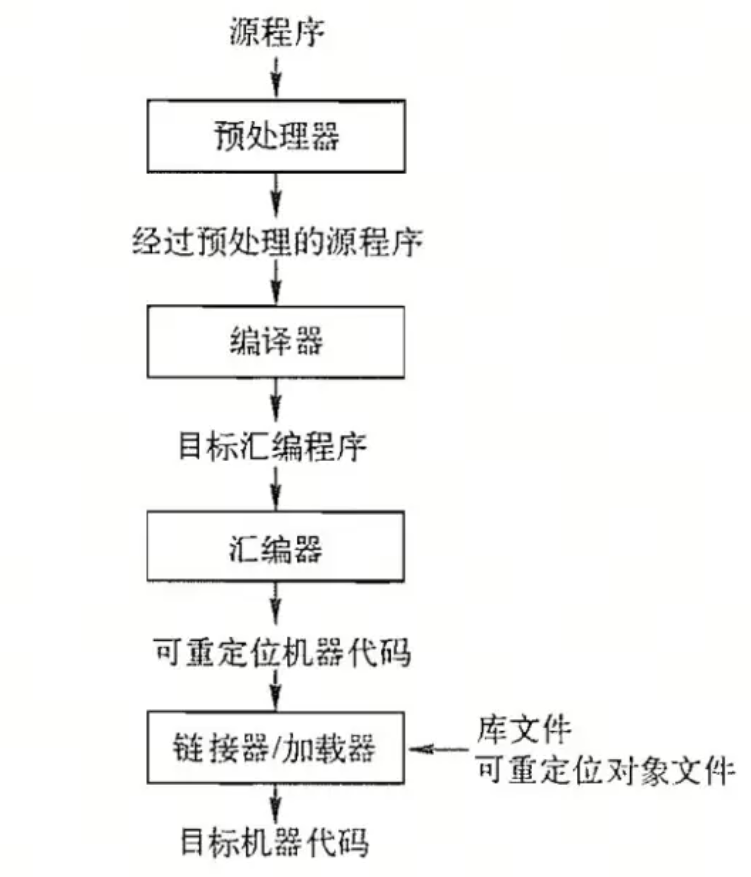
\includegraphics[width=10cm]{compile-process}
	\caption{源程序编译的一般过程}
\end{figure}

接下来我们逐步观察编译过程每一步的结果并对其展开分析。

\subsection{预处理器}
执行gcc factorial.c -E -o factorial.i 指令得到预处理结果。

观察factorial.i，从源代码的18行扩充到了831行，都多出了哪些代码？仔细观察，发现这些代码可以大致分为四类：

\begin{itemize}
	
	\item 标准库头文件的展开内容
	
	\begin{figure}[H]
		\centering	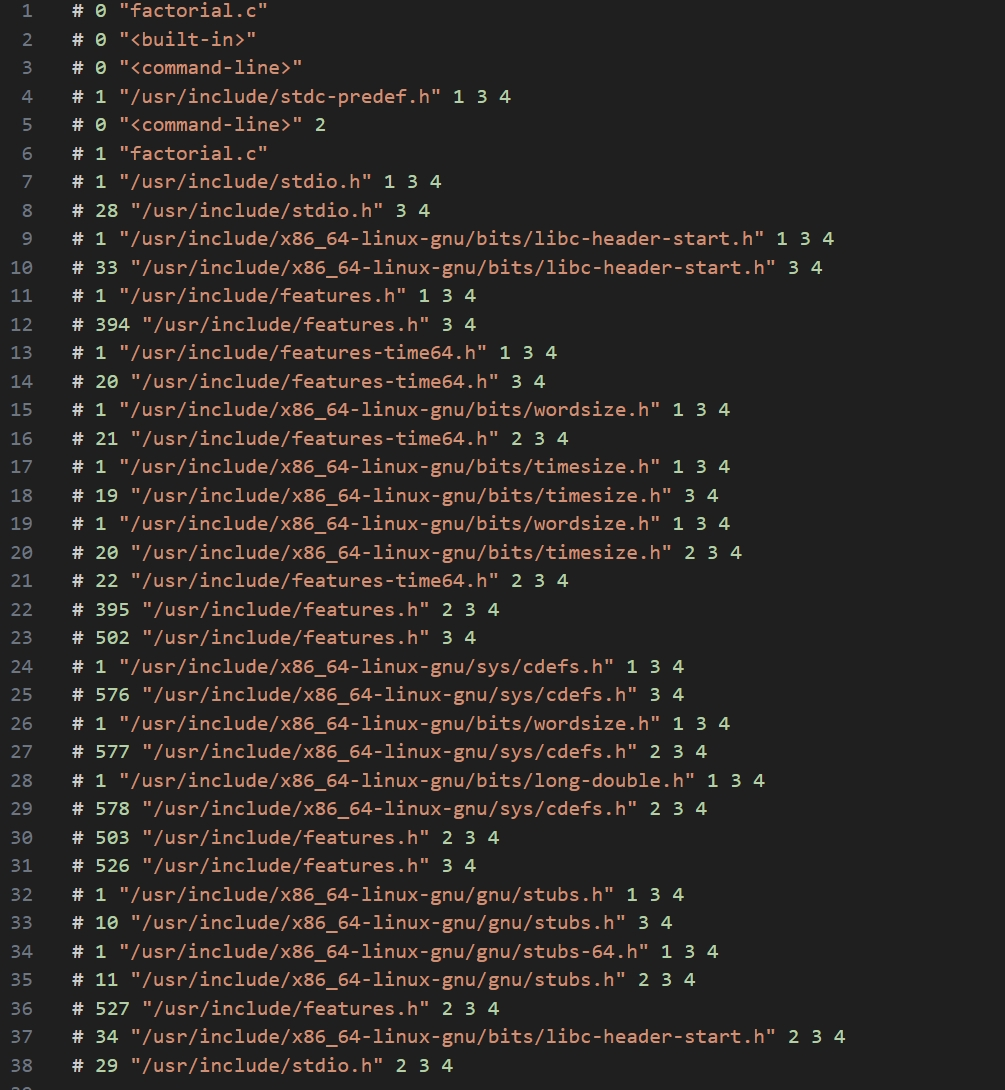
\includegraphics[width=10cm]{preprocess1}
		\caption{预处理结果——头文件展开}
	\end{figure}
	
	这些是在 factorial.c 中写的 \#include <stdio.h> ，预处理时被完整展开，把 stdio.h 及其嵌套的所有头文件源码都复制进来。它会继续 include： stdc-predef.h、features.h等等等等，所以行数暴增！
	仔细观察，这类代码大致可以划成以下结构：
	
	\# <行号> "<文件名>" <标志...>
	
	通过查阅网上的资料，这是GCC 预处理器生成的“行控制信息”，告诉编译器：当前行来自哪个源文件，行号是多少，标志各自有不同的含义，如：1：开始新的文件 2：回到上一个文件 3：以下文本来自系统头文件 4：应将下面的文本视为包含在隐式的外部“C”块中。
	
	提问：为什么会有？ 方便编译器在编译错误时仍能正确报告原始文件位置。
	
	\item 类型定义（typedef）
	
	\begin{figure}[H]
		\centering	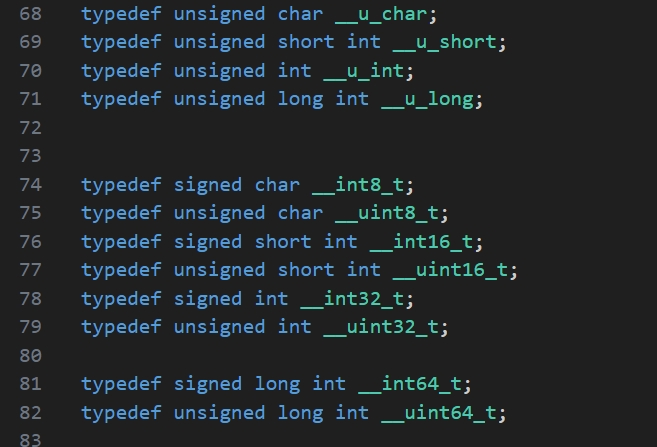
\includegraphics[width=10cm]{preprocess2}
		\caption{预处理结果——类型定义}
	\end{figure}
	
	这些代码来自各种头文件（尤其 stdint.h、types.h、libc 定义），用于给标准类型取别名，比如： \_\_int8\_t 变为 \_\_int\_least8\_t
	有什么用？用于平台无关性和兼容性
	
	\item 宏展开和函数声明
	
	\begin{figure}[H]
		\centering	
\includegraphics[width=10cm]{1}
		\caption{预处理结果——宏展开}
	\end{figure}
	\begin{figure}[H]
		\centering	
\includegraphics[width=10cm]{2}
		\caption{预处理结果——函数声明}
	\end{figure}
	
	诸如此类，这些代码来自 stdio.h 以及相关依赖，查资料可知预处理器会展开：内建宏、标准库声明、系统变量、I/O 结构体与函数声明
	
	\item 原始源码
	
	\begin{figure}[H]
		\centering	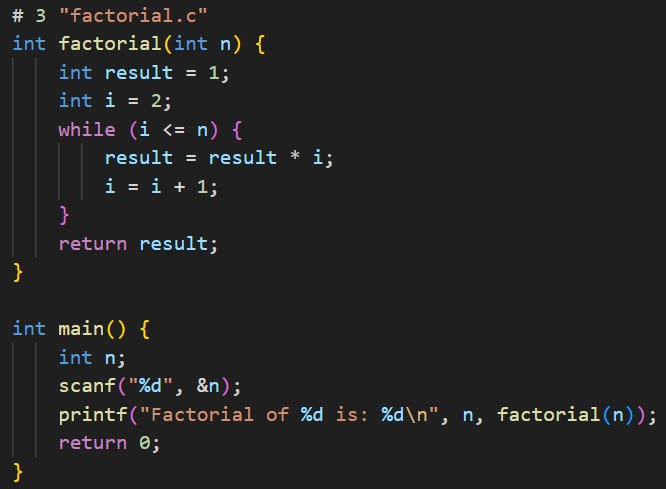
\includegraphics[width=10cm]{preprocess3}
		\caption{预处理结果——源码}
	\end{figure}
	
	在文件末尾找到了和源代码的函数定义以及main函数一模一样的代码块，只不过删除了注释。
\end{itemize}

根据观察以及网上资料，可以总结预处理器做了什么。

预处理器在编译器编译程序之前对源代码进行处理，通常分为以下几个阶段：

1.文件包含：处理 \#include 指令，将指定的头文件或代码文件插入到源代码中。

2.宏展开：对所有宏进行替换，将宏名称替换成对应的文本或表达式。

3.条件编译：根据条件编译指令 (\#ifdef, \#if 等) 来选择性地编译代码。

4.去除注释：删除源代码中的注释部分。

5.行号和调试信息：生成与行号、文件名等相关的调试信息。

最终，预处理器会生成一个新的源文件，这个文件会被传递给编译器进行编译。

\subsection{编译器}
在理论课程的学习中可知，编译的一般过程可以分为6步，分别是：

\begin{itemize}
	\item 词法分析
	\item 语法分析
	\item 语义分析
	\item 中间代码生成
	\item 代码优化
	\item 代码生成
\end{itemize}

接下来逐步执行编译步骤并对结果进行分析。

\subsubsection{词法分析}
执行 clang -E -Xclang -dump-tokens factorial.c 命令，可以得到词法分析的结果，截取部分结果如图：

\begin{figure}[H]
	\centering	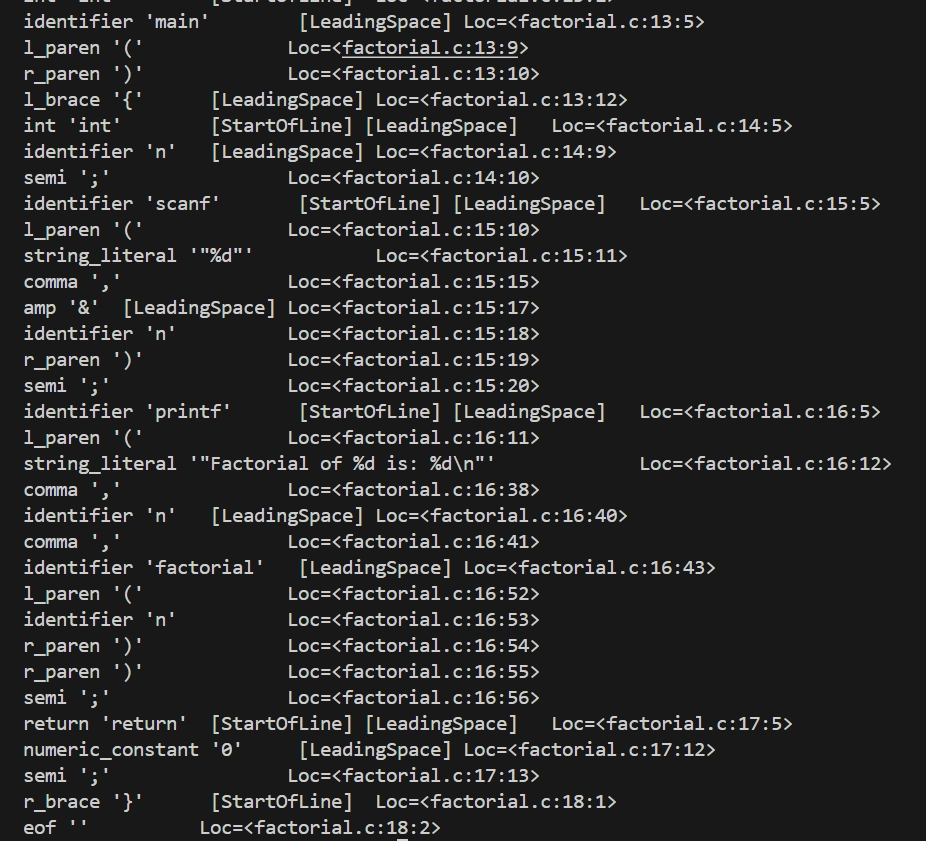
\includegraphics[width=10cm]{cifa}
	\caption{词法分析结果}
\end{figure}

观察输出，可以看到词法分析把文件分解成一个个 Token（词法单元），并为每个 Token 标注以下信息：
\begin{itemize}
	\item 词法类型（如 identifier、int、semi、l\_paren 等）
	\item 词面值（如 ferror\_unlocked、(、;、\_\_attribute\_\_ 等）
	\item 位置信息（Location）（文件名 + 行号 + 列号）
	\item 是否有前导空格、是否为行首、拼写来源等元信息（如 LeadingSpace、StartOfLine、Spelling）
\end{itemize}

仔细观察，大致可以为token归类：
\begin{table}[!htbp]
	\centering
	\begin{tabular}{ccccccccccc}
		\toprule  
		Token 类型& 示例& 用途\\
		\midrule
		关键字& int、while、return& 控制语句、类型声明\\
		标识符& factorial、FILE、\_\_stream& 变量、函数、宏\\
		常量& 1、0、2& 数字\\
		字符串字面量& "\%d"、"Factorial of \%d is: \%d \ n"& printf/scanf 参数\\
		运算符& +、*、=、<=& 表达式和赋值\\
		分隔符/界符& ( ) { } ,  ;  \& & 语句/参数边界\\
		属性标记& \_\_attribute\_\_, \_\_nothrow\_\_& GCC 扩展，来自头文件\\
		宏展开结果& 在 stdio.h 中被替换出的符号& <stdio.h> 展开后产生\\
		行控制信息(内部)& Spelling=/usr/include/...& 表示宏来自哪里\\
		\bottomrule
	\end{tabular}
	\caption{token归类}
	\label{table:t1}
\end{table}

\subsubsection{语法分析}

执行clang -E -Xclang -ast-dump factorial.c 命令进行语法分析，得到结果部分截图如下：
\begin{figure}[H]
	\centering	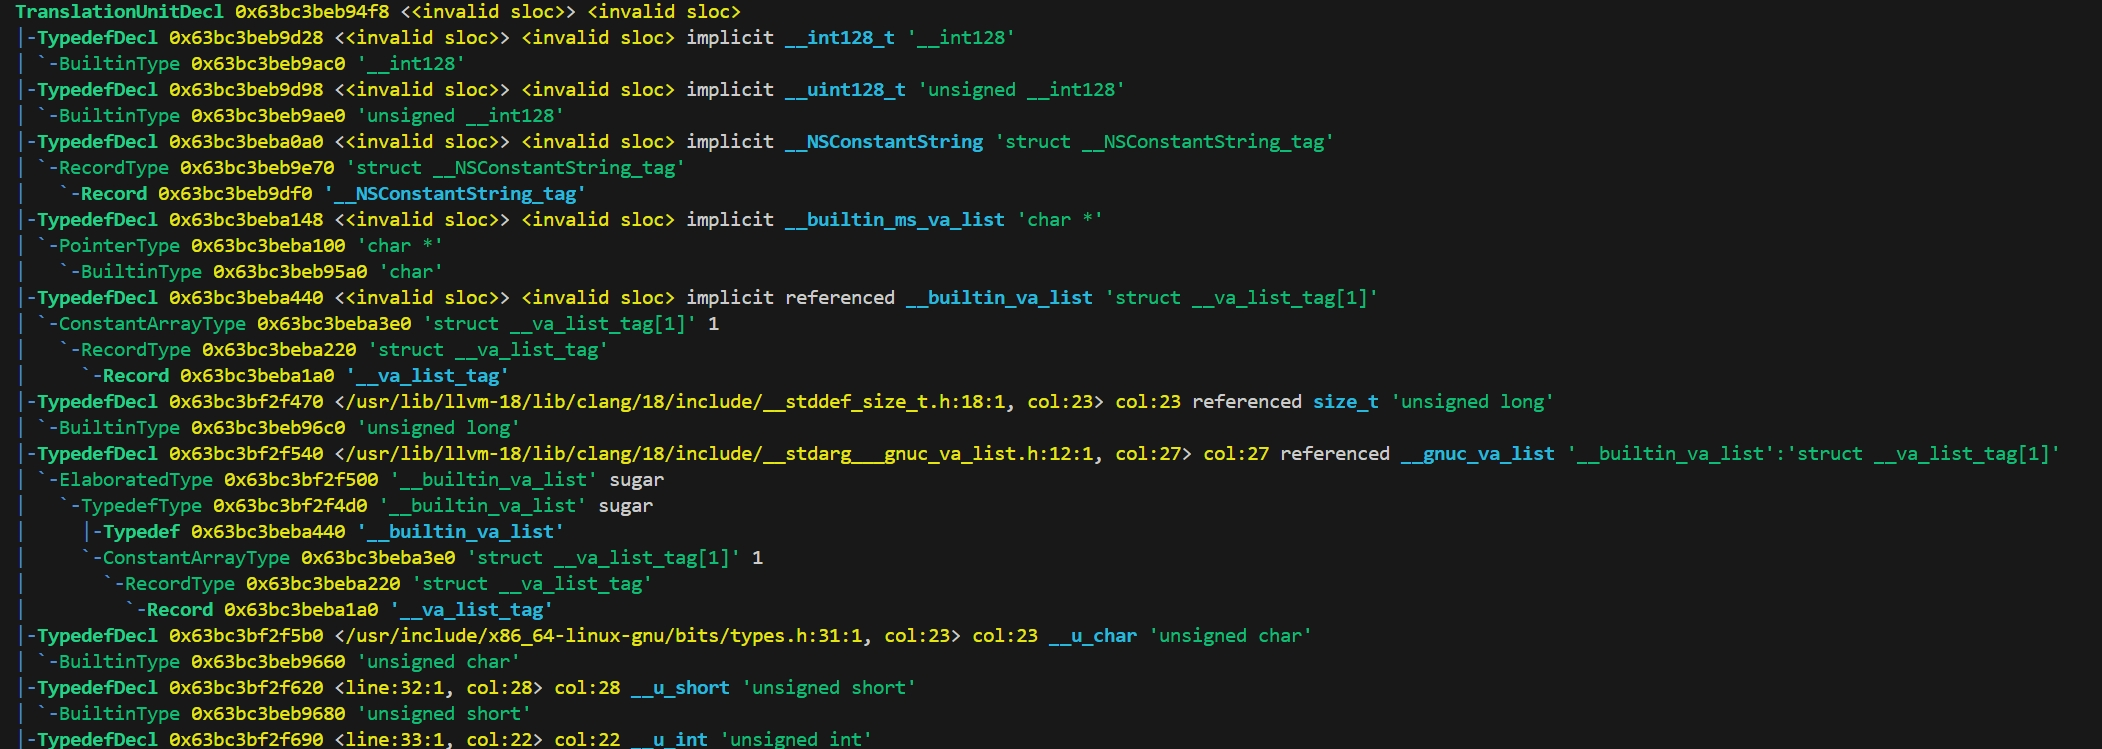
\includegraphics[width=10cm]{yufa}
	\caption{语法分析结果}
\end{figure}
让我们自顶向下观察生成的AST：

TranslationUnitDecl 是整个翻译单元（翻译单元＝预处理后的一整个源文件和被展开的头文件）的根节点。它下面列出很多 TypedefDecl / RecordDecl（来自系统头），以及源代码中函数 factorial 和 main 的 FunctionDecl 节点。

\paragraph{函数定义节点（FunctionDecl）}
以 factorial 为例，AST 中对应片段：
\begin{figure}[H]
	\centering	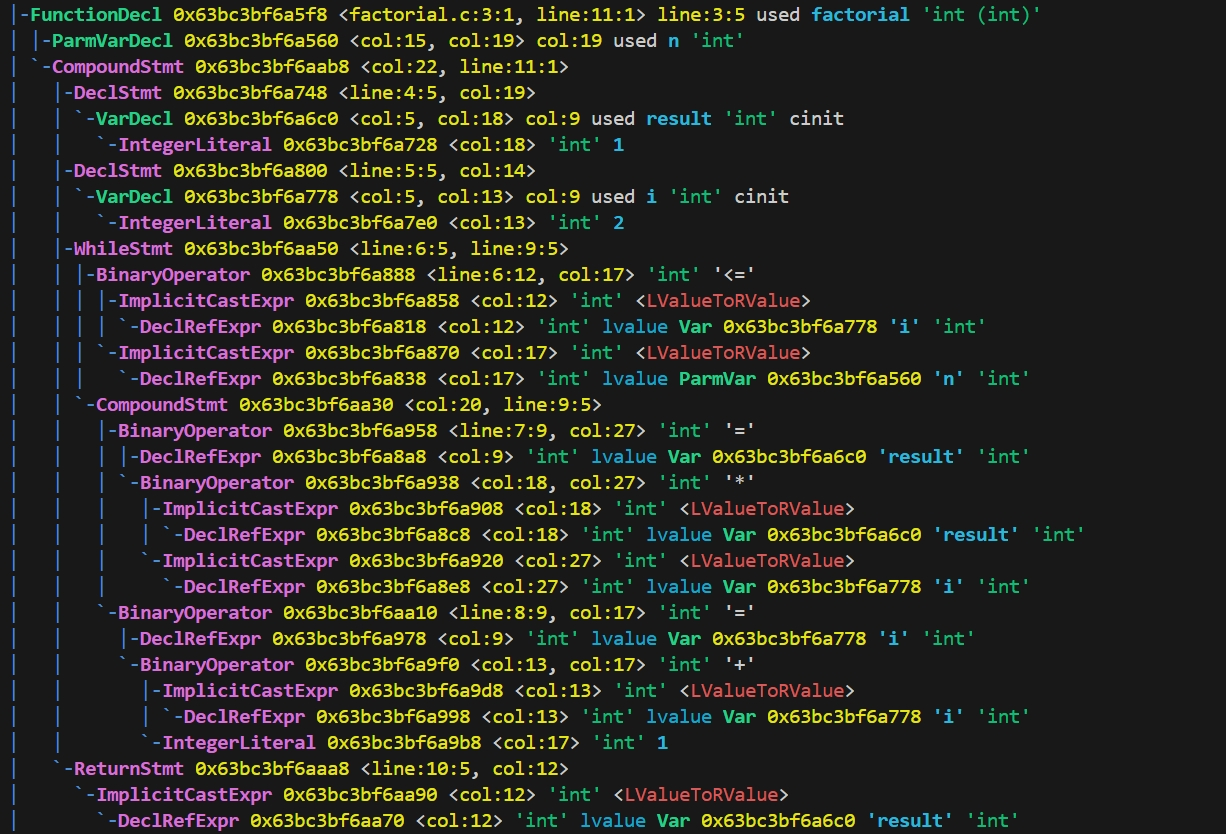
\includegraphics[width=10cm]{hanshu}
	\caption{函数定义节点}
\end{figure}
对比源代码，可以分析出语法分析树是怎么把原函数定义的信息变成AST节点的：
\begin{itemize}
	\item FunctionDecl：表示“函数的声明/定义”。节点带有位置信息（<factorial.c:3:1, line:11:1>），表示该函数从第 3 行第 1 列开始，到第 11 行结束，用于定位源代码。
	节点后面 'int (int)' 表示函数类型（返回 int，形参为 int）。
	used、implicit、extern 等是 clang 的附加标记，表示是否被使用、是否隐式生成等。
	\item ParmVarDecl：表示形参（这里是 n），有类型（int）和位置信息。
	\item CompoundStmt：表示函数体的大括号 { ... }，它的子节点依次是局部变量声明 (DeclStmt/VarDecl)、控制流语句（WhileStmt）、以及返回语句（ReturnStmt）。
	\item VarDecl ... cinit IntegerLiteral： VarDecl 描述局部变量（如 result、i）。cinit 表示带有初始化表达式；初始化子节点是 IntegerLiteral 1 或 2。
\end{itemize}

\paragraph{语句节点}
\begin{itemize}
	\item WhileStmt（循环）
	\begin{figure}[H]
		\centering	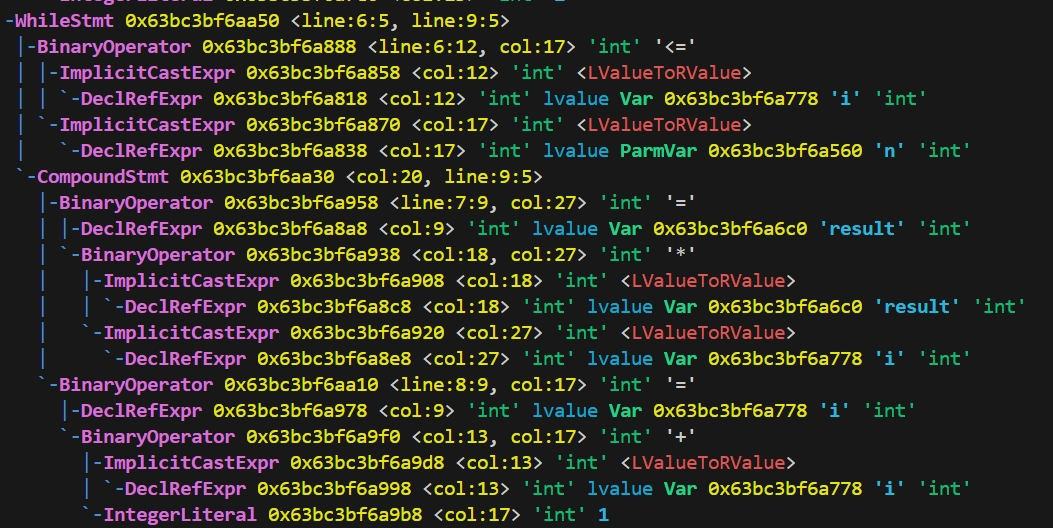
\includegraphics[width=10cm]{xunhuan}
		\caption{循环语句节点}
	\end{figure}
	WhileStmt 节点有两个重要子节点：
	1.条件表达式（这里是 BinaryOperator '<='）——判断 i <= n。
	条件的左右是 DeclRefExpr（对变量的引用），通常被 ImplicitCastExpr 包裹（把 LValue 转成 RValue）。
	2.循环体（CompoundStmt）——循环内的语句列表。每一条语句在 AST 中仍然有自己的节点，例如赋值是 BinaryOperator '='。
	\item ReturnStmt（返回语句）
	\begin{figure}[H]
		\centering	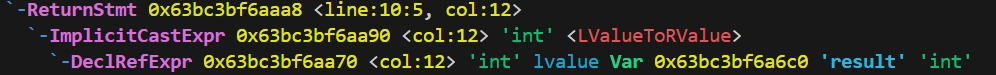
\includegraphics[width=10cm]{fanhui}
		\caption{返回语句节点}
	\end{figure}
	表示 return result; DeclRefExpr 表示对 result 的引用，ImplicitCastExpr 把左值转换成右值以便返回。
\end{itemize}

\paragraph{表达式节点（算术运算 / 函数调用 / 隐式转换）}
1.算术运算不再赘述
2.CallExpr（函数调用）
\begin{figure}[H]
	\centering	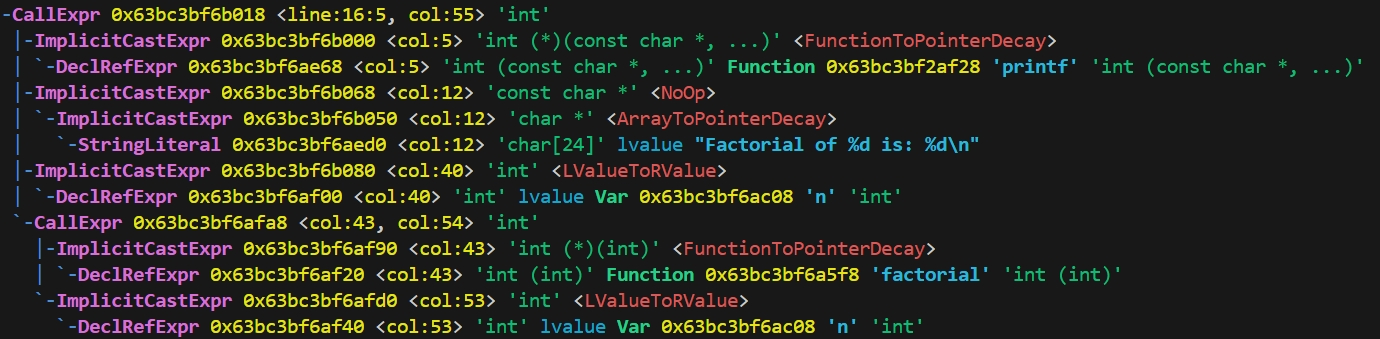
\includegraphics[width=10cm]{diaoyong}
	\caption{函数调用节点}
\end{figure}
CallExpr 是函数调用节点。第一个子节点通常是函数表达式（DeclRefExpr，在需要时外面包 ImplicitCastExpr 做 FunctionToPointerDecay），之后是各个参数表达式。
可以注意到 factorial(n) 在 printf 的参数中以一个 子 CallExpr 的形式出现：AST 支持任意嵌套表达式。
3.ImplicitCastExpr（隐式类型转换）
可以频繁看到 ImplicitCastExpr，常见的转换类型包括：
\begin{itemize}
	\item <LValueToRValue>：把变量的左值（lvalue）转换为右值（rvalue），例如在表达式中读取变量的值。大量出现在算术操作和参数传递处。
	\item <FunctionToPointerDecay>：函数名在调用处从函数类型退化为函数指针（scanf/printf/factorial 的节点里可见）。
	\item <ArrayToPointerDecay>：字符串字面量或数组名在做参数时退化为指针（例如 StringLiteral 被 ArrayToPointerDecay 包裹，再可能被 NoOp 转为 const char *）。
	\item <NoOp>：类型无需调整但是 AST 仍显示一个“无操作”转换（常见于 char * -> const char * 的 const 加装）。
\end{itemize}
这些隐式类型转换为什么重要？
这些隐式转换节点记录了编译器在语义层面做的类型调整，后续生成 IR / 代码时要根据这些信息插入适当的读取/转换指令。

\subsubsection{语义分析}

在上一步生成的语法分析中其实已经进行了语义分析处理，不再赘述。

\subsubsection{中间代码生成}
执行clang -S -emit-llvm factorial.c -o factorial.ll 命令生成LLVM IR文件: factorial.ll。
接下来分析一下LLVM IR结构：

\paragraph{模块头}
\lstset{
	columns=fixed,       
	numbers=left,                                        % 在左侧显示行号
	numberstyle=\tiny\color{gray},                       % 设定行号格式
	frame=none,                                          % 不显示背景边框
	backgroundcolor=\color[RGB]{245,245,244},            % 设定背景颜色
	keywordstyle=\color[RGB]{40,40,255},                 % 设定关键字颜色
	numberstyle=\footnotesize\color{darkgray},           
	commentstyle=\it\color[RGB]{0,96,96},                % 设置代码注释的格式
	stringstyle=\rmfamily\slshape\color[RGB]{128,0,0},   % 设置字符串格式
	showstringspaces=false,                              % 不显示字符串中的空格
	language=LLVM,                                        % 设置语言
}
\begin{lstlisting}
	; ModuleID = 'factorial.c'
	source_filename = "factorial.c"
	target datalayout = "e-m:e-p270:32:32-p271:32:32-p272:64:64-i64:64-i128:128-f80:128-n8:16:32:64-S128"
	target triple = "x86_64-pc-linux-gnu"
\end{lstlisting}
ModuleID / source\_filename：模块与源文件标识。

target datalayout：目标机器的数据对齐与内存布局规则（整数/浮点宽度、对齐、指针大小等）。生成的 IR 必须遵守这些规则以便后端生成正确机器码。

target triple：目标架构和平台，影响 ABI、调用约定等。

\paragraph{全局常量（字符串字面量）}
\lstset{
	columns=fixed,       
	numbers=left,                                        % 在左侧显示行号
	numberstyle=\tiny\color{gray},                       % 设定行号格式
	frame=none,                                          % 不显示背景边框
	backgroundcolor=\color[RGB]{245,245,244},            % 设定背景颜色
	keywordstyle=\color[RGB]{40,40,255},                 % 设定关键字颜色
	numberstyle=\footnotesize\color{darkgray},           
	commentstyle=\it\color[RGB]{0,96,96},                % 设置代码注释的格式
	stringstyle=\rmfamily\slshape\color[RGB]{128,0,0},   % 设置字符串格式
	showstringspaces=false,                              % 不显示字符串中的空格
	language=LLVM,                                        % 设置语言
}
\begin{lstlisting}
	@.str = private unnamed_addr constant [3 x i8] c"%d\00", align 1
	@.str.1 = private unnamed_addr constant [24 x i8] c"Factorial of %d is: %d\0A\00", align 1
\end{lstlisting}
原 C 中的 "\%d" 和 "Factorial of \%d is: \%d \textbackslash n" 被放在程序的只读数据区（全局常量），用数组类型 [N x i8] 表示每个字符并以 \textbackslash00 结尾。

这样 scanf/printf 在运行时可以接收指向这些内存的指针作为格式字符串参数。

private unnamed\_addr 等表示链接可见性与地址不关心（优化提示）。

\paragraph{函数定义：@factorial 的 IR}
\lstset{
	columns=fixed,       
	numbers=left,                                        % 在左侧显示行号
	numberstyle=\tiny\color{gray},                       % 设定行号格式
	frame=none,                                          % 不显示背景边框
	backgroundcolor=\color[RGB]{245,245,244},            % 设定背景颜色
	keywordstyle=\color[RGB]{40,40,255},                 % 设定关键字颜色
	numberstyle=\footnotesize\color{darkgray},           
	commentstyle=\it\color[RGB]{0,96,96},                % 设置代码注释的格式
	stringstyle=\rmfamily\slshape\color[RGB]{128,0,0},   % 设置字符串格式
	showstringspaces=false,                              % 不显示字符串中的空格
	language=LLVM,                                        % 设置语言
}
\begin{lstlisting}
	define dso_local i32 @factorial(i32 noundef %0) #0 {
		%2 = alloca i32, align 4        ; stack slot for param n (saved)
		%3 = alloca i32, align 4        ; stack slot for result
		%4 = alloca i32, align 4        ; stack slot for i
		store i32 %0, ptr %2, align 4   ; store argument into %2
		store i32 1, ptr %3, align 4    ; result = 1
		store i32 2, ptr %4, align 4    ; i = 2
		br label %5                     ; jump to loop-test block
		5:
		%6 = load i32, ptr %4, align 4
		%7 = load i32, ptr %2, align 4
		%8 = icmp sle i32 %6, %7
		br i1 %8, label %9, label %15   ; if (i <= n) goto body else goto exit
		9:
		%10 = load i32, ptr %3, align 4
		%11 = load i32, ptr %4, align 4
		%12 = mul nsw i32 %10, %11
		store i32 %12, ptr %3, align 4  ; result = result * i
		%13 = load i32, ptr %4, align 4
		%14 = add nsw i32 %13, 1
		store i32 %14, ptr %4, align 4  ; i = i + 1
		br label %5, !llvm.loop !6      ; jump back to test (loop metadata)
		15:
		%16 = load i32, ptr %3, align 4
		ret i32 %16
	}
\end{lstlisting}
\begin{itemize}
	\item alloca（栈上分配） 
	
	每个局部变量（包括编译器将函数参数拷贝到的“本地槽”）在函数入口用 alloca 分配栈空间。
	AI提示，这是典型的 -O0（未优化）策略：变量保存在内存里，方便逐步调试（与寄存器机械式保存相比更容易与源代码一一对应）。 因为IR 包含大量 load/store 而没有 SSA φ 节点，说明编译器选择把变量保持在内存（不是寄存器）——这是由 optnone（未优化）影响的常见结果。
	\item 将参数存入栈
	
	\%0 是函数参数（直接传入的寄存器或栈位置），第一件事即 store \%0, \%2，把它拷入本地槽 \%2（这样后面用 load \%2 得到 n 的值）。这保证调试时 \%2 与源代码变量 n 一一对应。
	\item 分支/基本块
	
	br label \%5、br i1 \%8, label \%9, label \%15 表示基本块之间的控制流。编号（5、9、15）只是 LLVM 为基本块生成的符号。
	
	\%8 = icmp sle i32 \%6, \%7 对应 i <= n 条件判断。icmp 是整数比较（signed less-or-equal）。
	
	\item 算术运算 mul nsw、add nsw
	
	mul nsw i32 \%10, \%11 表示带 NSW（No Signed Wrap） 的乘法：此运算假定带符号整数溢出不发生（若发生则行为未定义），编译器可据此进行某些优化（但在 -O0 并未利用）。
	add nsw i32 \%13, 1 同理。
	\item !llvm.loop !6（loop metadata）
	
	这是循环元数据（后面文件有 !6 = distinct !{!6, !7} 和 !7 = !"llvm.loop.mustprogress"），表示循环相关属性（例如必须有进展等），有助于后续的 loop 优化分析。
\end{itemize}

\paragraph{@main 的 IR}
\lstset{
	columns=fixed,       
	numbers=left,                                        % 在左侧显示行号
	numberstyle=\tiny\color{gray},                       % 设定行号格式
	frame=none,                                          % 不显示背景边框
	backgroundcolor=\color[RGB]{245,245,244},            % 设定背景颜色
	keywordstyle=\color[RGB]{40,40,255},                 % 设定关键字颜色
	numberstyle=\footnotesize\color{darkgray},           
	commentstyle=\it\color[RGB]{0,96,96},                % 设置代码注释的格式
	stringstyle=\rmfamily\slshape\color[RGB]{128,0,0},   % 设置字符串格式
	showstringspaces=false,                              % 不显示字符串中的空格
	language=LLVM,                                        % 设置语言
}
\begin{lstlisting}
	define dso_local i32 @main() #0 {
		%1 = alloca i32, align 4
		%2 = alloca i32, align 4
		store i32 0, ptr %1, align 4
		%3 = call i32 (ptr, ...) @__isoc99_scanf(ptr noundef @.str, ptr noundef %2)
		%4 = load i32, ptr %2, align 4
		%5 = load i32, ptr %2, align 4
		%6 = call i32 @factorial(i32 noundef %5)
		%7 = call i32 (ptr, ...) @printf(ptr noundef @.str.1, i32 noundef %4, i32 noundef %6)
		ret i32 0
	}
\end{lstlisting}
\%2 是 n 的栈槽（用于 scanf 写入）。scanf 被调用时传入 @.str（格式字符串全局地址）和 \%2 的指针（ptr noundef \%2）。

load 两次（\%4、\%5）都是把 n 的值从内存读出来——这里重复读取用于传递给 printf 的第一个参数和传给 factorial 的参数。编译器在 -O0 不做冗余消除，所以出现重复 load。

调用 @factorial：call i32 @factorial(i32 noundef \%5)，把刚才加载的 n 传入。
printf：以格式字符串与两个整型参数（n、factorial(n) 的返回值）调用。
最后 ret i32 0：返回 0（main 的返回值）。

\paragraph{函数声明（外部可变参数函数）}
\lstset{
	columns=fixed,       
	numbers=left,                                        % 在左侧显示行号
	numberstyle=\tiny\color{gray},                       % 设定行号格式
	frame=none,                                          % 不显示背景边框
	backgroundcolor=\color[RGB]{245,245,244},            % 设定背景颜色
	keywordstyle=\color[RGB]{40,40,255},                 % 设定关键字颜色
	numberstyle=\footnotesize\color{darkgray},           
	commentstyle=\it\color[RGB]{0,96,96},                % 设置代码注释的格式
	stringstyle=\rmfamily\slshape\color[RGB]{128,0,0},   % 设置字符串格式
	showstringspaces=false,                              % 不显示字符串中的空格
	language=LLVM,                                        % 设置语言
}
\begin{lstlisting}
	declare i32 @__isoc99_scanf(ptr noundef, ...) #1
	declare i32 @printf(ptr noundef, ...) #1
\end{lstlisting}
declare 表示外部函数的原型（没有定义体）。格式 i32 (ptr, ...) 标明这些函数是可变参数（vararg）的 C 库函数，LLVM 必须按目标平台 ABI 为 vararg 调用生成正确的参数传递代码（例如寄存器/栈使用）。

属性集合 \#1（在后面有定义）包含与目标相关的属性（frame-pointer、no-trapping-math 等）。

\paragraph{属性（attributes）与模块元数据}
\lstset{
	columns=fixed,       
	numbers=left,                                        % 在左侧显示行号
	numberstyle=\tiny\color{gray},                       % 设定行号格式
	frame=none,                                          % 不显示背景边框
	backgroundcolor=\color[RGB]{245,245,244},            % 设定背景颜色
	keywordstyle=\color[RGB]{40,40,255},                 % 设定关键字颜色
	numberstyle=\footnotesize\color{darkgray},           
	commentstyle=\it\color[RGB]{0,96,96},                % 设置代码注释的格式
	stringstyle=\rmfamily\slshape\color[RGB]{128,0,0},   % 设置字符串格式
	showstringspaces=false,                              % 不显示字符串中的空格
	language=LLVM,                                        % 设置语言
}
\begin{lstlisting}
	attributes #0 = { noinline nounwind optnone uwtable "frame-pointer"="all" "min-legal-vector-width"="0" "no-trapping-math"="true" "stack-protector-buffer-size"="8" "target-cpu"="x86-64" "target-features"="+cmov,+cx8,+fxsr,+mmx,+sse,+sse2,+x87" "tune-cpu"="generic" }
	attributes #1 = { "frame-pointer"="all" "no-trapping-math"="true" "stack-protector-buffer-size"="8" "target-cpu"="x86-64" "target-features"="+cmov,+cx8,+fxsr,+mmx,+sse,+sse2,+x87" "tune-cpu"="generic" }
	
	!llvm.module.flags = !{!0, !1, !2, !3, !4}
	!llvm.ident = !{!5}
	
	!0 = !{i32 1, !"wchar_size", i32 4}
	!1 = !{i32 8, !"PIC Level", i32 2}
	!2 = !{i32 7, !"PIE Level", i32 2}
	!3 = !{i32 7, !"uwtable", i32 2}
	!4 = !{i32 7, !"frame-pointer", i32 2}
	!5 = !{!"Ubuntu clang version 18.1.3 (1ubuntu1)"}
	!6 = distinct !{!6, !7}
	!7 = !{!"llvm.loop.mustprogress"}
\end{lstlisting}
\begin{itemize}
	\item noinline：
	
	不要内联（对于 -O0，保持可见函数边界便于调试）。
	\item nounwind：
	
	函数不会抛出 C++ 异常。
	\item optnone：
	
	禁止优化（常见于 -O0，保留源码结构用于调试）。
	\item uwtable：
	
	生成 unwind table（异常/栈展开信息），对调试与栈回溯有用。
	\item 模块 flags（PIC Level、PIE Level、frame-pointer 等）
	
	记录了编译目标/选项信息。
	\item !llvm.loop.mustprogress：
	
	标记循环必须进展，避免无限循环的某些优化假设被破坏。
\end{itemize}

\paragraph{总结}
中间代码是前端（语法/语义分析）和后端（目标机器代码生成）之间的跨平台、可优化的中间抽象层，用于表示程序的语义与控制流，使得大量与目标无关的分析与优化可以统一、重复地执行，把语言语义与目标平台解耦，然后再lower到具体机器指令。


\subsubsection{代码生成}
执行 aarch64-linux-gnu-gcc factorial.i -S -o factorial.S 命令，以中间表示形式作为输入，将其映射到目标语言。

观察生成的汇编语言，可以分析编译器在这阶段做了什么：

\begin{itemize}
	\item 把“架构无关的中间代码”转换成“目标机器相关的汇编指令”
	
	LLVM IR 或内部 SSA 表示的运算、控制流、函数调用、变量访问，会被降级为具体 CPU 指令集的操作。
	\begin{figure}[H]
		\centering	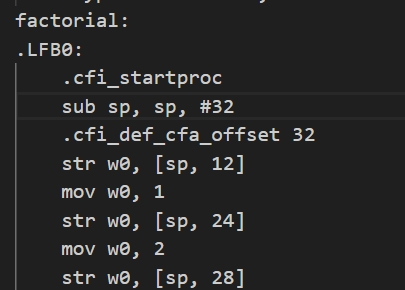
\includegraphics[width=10cm]{mubiao1}
	\end{figure}
	上图对应的源代码：
	\lstset{
		columns=fixed,       
		numbers=left,                                        % 在左侧显示行号
		numberstyle=\tiny\color{gray},                       % 设定行号格式
		frame=none,                                          % 不显示背景边框
		backgroundcolor=\color[RGB]{245,245,244},            % 设定背景颜色
		keywordstyle=\color[RGB]{40,40,255},                 % 设定关键字颜色
		numberstyle=\footnotesize\color{darkgray},           
		commentstyle=\it\color[RGB]{0,96,96},                % 设置代码注释的格式
		stringstyle=\rmfamily\slshape\color[RGB]{128,0,0},   % 设置字符串格式
		showstringspaces=false,                              % 不显示字符串中的空格
		language=c,                                        % 设置语言
	}
	\begin{lstlisting}
		int factorial(int n) {
			int result = 1;
			int i = 2;
	\end{lstlisting}
	可见进行了变量分配与栈帧建立。
	\item 控制流结构变成跳转和标签
	\begin{figure}[H]
		\centering	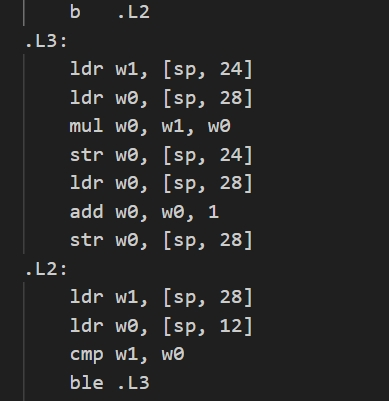
\includegraphics[width=10cm]{mubiao2}
	\end{figure}
	这里对应的是源码里的一处while循环，.L2 / .L3 是基本块标签，cmp + ble 实现 <= 分支控制。
	\item 算术表达式变为机器指令
	
	例如：
	\lstset{
		columns=fixed,       
		numbers=left,                                        % 在左侧显示行号
		numberstyle=\tiny\color{gray},                       % 设定行号格式
		frame=none,                                          % 不显示背景边框
		backgroundcolor=\color[RGB]{245,245,244},            % 设定背景颜色
		keywordstyle=\color[RGB]{40,40,255},                 % 设定关键字颜色
		numberstyle=\footnotesize\color{darkgray},           
		commentstyle=\it\color[RGB]{0,96,96},                % 设置代码注释的格式
		stringstyle=\rmfamily\slshape\color[RGB]{128,0,0},   % 设置字符串格式
		showstringspaces=false,                              % 不显示字符串中的空格
		language=c,                                        % 设置语言
	}
	\begin{lstlisting}
		mul	w0, w1, w0   ; result * i
		add	w0, w0, 1    ; i = i + 1
	\end{lstlisting}
	\item 函数调用使用 ABI 调用约定
	
	调用 factorial、printf、scanf时，GCC 遵循 ARM64 ABI：
	参数放在寄存器：x0, x1, x2, ...
	返回值在 w0 / x0
	\item 字符串常量放入 .rodata 段
	\lstset{
		columns=fixed,       
		numbers=left,                                        % 在左侧显示行号
		numberstyle=\tiny\color{gray},                       % 设定行号格式
		frame=none,                                          % 不显示背景边框
		backgroundcolor=\color[RGB]{245,245,244},            % 设定背景颜色
		keywordstyle=\color[RGB]{40,40,255},                 % 设定关键字颜色
		numberstyle=\footnotesize\color{darkgray},           
		commentstyle=\it\color[RGB]{0,96,96},                % 设置代码注释的格式
		stringstyle=\rmfamily\slshape\color[RGB]{128,0,0},   % 设置字符串格式
		showstringspaces=false,                              % 不显示字符串中的空格
		language=c,                                        % 设置语言
	}
	\begin{lstlisting}
		.section	.rodata
		.LC0:
				.string	"%d"
	\end{lstlisting}
	把 C 的格式字符串静态放入只读内存，并通过 adrp + add 访问。
	\item 主函数多了栈保护
	
	可以观察到main 函数中有额外逻辑：
	\lstset{
		columns=fixed,       
		numbers=left,                                        % 在左侧显示行号
		numberstyle=\tiny\color{gray},                       % 设定行号格式
		frame=none,                                          % 不显示背景边框
		backgroundcolor=\color[RGB]{245,245,244},            % 设定背景颜色
		keywordstyle=\color[RGB]{40,40,255},                 % 设定关键字颜色
		numberstyle=\footnotesize\color{darkgray},           
		commentstyle=\it\color[RGB]{0,96,96},                % 设置代码注释的格式
		stringstyle=\rmfamily\slshape\color[RGB]{128,0,0},   % 设置字符串格式
		showstringspaces=false,                              % 不显示字符串中的空格
		language=c,                                        % 设置语言
	}
	\begin{lstlisting}
		adrp	x0, :got:__stack_chk_guard
		ldr	x0, [x0, :got_lo12:__stack_chk_guard]
		ldr	x1, [x0]
		str	x1, [sp, 8]
		...
		ldr	x3, [sp, 8]
		ldr	x2, [x0]
		subs	x3, x3, x2
		beq	.L7
		bl	__stack_chk_fail
	\end{lstlisting}
	结合AI分析，这是 GCC 自动加入的栈溢出保护机制（默认开启 -fstack-protector）。
	\item 符号定义与可链接信息生成
	\lstset{
		columns=fixed,       
		numbers=left,                                        % 在左侧显示行号
		numberstyle=\tiny\color{gray},                       % 设定行号格式
		frame=none,                                          % 不显示背景边框
		backgroundcolor=\color[RGB]{245,245,244},            % 设定背景颜色
		keywordstyle=\color[RGB]{40,40,255},                 % 设定关键字颜色
		numberstyle=\footnotesize\color{darkgray},           
		commentstyle=\it\color[RGB]{0,96,96},                % 设置代码注释的格式
		stringstyle=\rmfamily\slshape\color[RGB]{128,0,0},   % 设置字符串格式
		showstringspaces=false,                              % 不显示字符串中的空格
		language=c,                                        % 设置语言
	}
	\begin{lstlisting}
		.global factorial
		.type factorial, %function
		.size factorial, .-factorial
	\end{lstlisting}
	这些告诉链接器：哪些函数是外部可见的、它们的范围和地址、需要如何组织可执行文件
	\item 函数栈结构与调试信息
	\lstset{
		columns=fixed,       
		numbers=left,                                        % 在左侧显示行号
		numberstyle=\tiny\color{gray},                       % 设定行号格式
		frame=none,                                          % 不显示背景边框
		backgroundcolor=\color[RGB]{245,245,244},            % 设定背景颜色
		keywordstyle=\color[RGB]{40,40,255},                 % 设定关键字颜色
		numberstyle=\footnotesize\color{darkgray},           
		commentstyle=\it\color[RGB]{0,96,96},                % 设置代码注释的格式
		stringstyle=\rmfamily\slshape\color[RGB]{128,0,0},   % 设置字符串格式
		showstringspaces=false,                              % 不显示字符串中的空格
		language=c,                                        % 设置语言
	}
	\begin{lstlisting}
		.cfi_startproc
		.cfi_offset 29, -32
		.cfi_endproc
	\end{lstlisting}
	这些是 调用帧信息 (CFI)，用于调试器和异常回溯。
\end{itemize}


\subsection{汇编器——目标文件生成}
执行 aarch64-linux-gnu-gcc factorial.S -c -o factorial.o命令进行交叉编译，把汇编语言程序代码翻译成目标机器指令，最终生成可重定位的机器代码。

由于二进制文件不易分析，我又执行了 aarch64-linux-gnu-objdump -d factorial.o > factorial-obj-disasm.s 和 nm factorial.o > factorial-obj-symbols.txt 生成了反汇编文件和符号表，以此分析汇编器的工作和功能：

\subsubsection{从反汇编文件看汇编器输出}
反汇编显示的格式是：

<offset> <machine-code-bytes> <asm-instruction>。

因为这是可重定位目标文件，所有地址/相对位移都是节内偏移 / 占位，真正的绝对地址要留待链接器修正。

\begin{itemize}
	\item 函数前序：栈帧/局部变量分配
	
	\lstset{
		columns=fixed,       
		numbers=left,                                        % 在左侧显示行号
		numberstyle=\tiny\color{gray},                       % 设定行号格式
		frame=none,                                          % 不显示背景边框
		backgroundcolor=\color[RGB]{245,245,244},            % 设定背景颜色
		keywordstyle=\color[RGB]{40,40,255},                 % 设定关键字颜色
		numberstyle=\footnotesize\color{darkgray},           
		commentstyle=\it\color[RGB]{0,96,96},                % 设置代码注释的格式
		stringstyle=\rmfamily\slshape\color[RGB]{128,0,0},   % 设置字符串格式
		showstringspaces=false,                              % 不显示字符串中的空格
		language=c,                                        % 设置语言
	}
	\begin{lstlisting}
		00000000 <factorial>:
		0: d10083ff  sub sp, sp, #0x20
		4: b9000fe0  str w0, [sp, #12]
		...
		48: b9401be0 	ldr w0, [sp, #24]
		4c: 910083ff  add sp, sp, #0x20
		50: d65f03c0  ret
	\end{lstlisting}
	汇编器把函数抽象（局部变量）映射成具体栈偏移的 str/ldr 操作，生成函数头尾（ prologue/epilogue） 保证 ABI 与栈平衡。
	\item 循环与条件分支的翻译（控制流）
	
	\lstset{
		columns=fixed,       
		numbers=left,                                        % 在左侧显示行号
		numberstyle=\tiny\color{gray},                       % 设定行号格式
		frame=none,                                          % 不显示背景边框
		backgroundcolor=\color[RGB]{245,245,244},            % 设定背景颜色
		keywordstyle=\color[RGB]{40,40,255},                 % 设定关键字颜色
		numberstyle=\footnotesize\color{darkgray},           
		commentstyle=\it\color[RGB]{0,96,96},                % 设置代码注释的格式
		stringstyle=\rmfamily\slshape\color[RGB]{128,0,0},   % 设置字符串格式
		showstringspaces=false,                              % 不显示字符串中的空格
		language=c,                                        % 设置语言
	}
	\begin{lstlisting}
		 18: 14000008  b 38 <factorial+0x38>
		1c: b9401be1  ldr w1, [sp, #24]
		20: b9401fe0  ldr w0, [sp, #28]
		24: 1b007c20  mul w0, w1, w0
		...
		38: b9401fe1  ldr w1, [sp, #28]
		3c: b9400fe0  ldr w0, [sp, #12]
		40: 6b00003f  cmp w1, w0
		44: 54fffecd  b.le 1c <factorial+0x1c>
	\end{lstlisting}
	观察反汇编，这段代码通过翻译b和b.le实现 while (i <= n) 控制流。控制流的基本块在目标代码中以标签（offset）表示，分支是机器跳转指令。
	\item 主函数中：调用约定、全局/常量引用、栈保护
	\item 地址/常量的生成：adrp + add / GOT 访问
	
	在 AArch64，访问远距离的全局地址通常用 adrp（把页基地址加载到寄存器）配合 add（加上页内偏移），或 adrp + ldr [x0, :got\_lo12:] 之类的序列。因为 .o 仍是可重定位的，adrp 的立即数/补位不是最终值，链接器会对这些指令产生重定位修正。
\end{itemize}

\subsubsection{从 nm 的符号表看：符号的种类与链接责任}
\lstset{
	columns=fixed,       
	numbers=left,                                        % 在左侧显示行号
	numberstyle=\tiny\color{gray},                       % 设定行号格式
	frame=none,                                          % 不显示背景边框
	backgroundcolor=\color[RGB]{245,245,244},            % 设定背景颜色
	keywordstyle=\color[RGB]{40,40,255},                 % 设定关键字颜色
	numberstyle=\footnotesize\color{darkgray},           
	commentstyle=\it\color[RGB]{0,96,96},                % 设置代码注释的格式
	stringstyle=\rmfamily\slshape\color[RGB]{128,0,0},   % 设置字符串格式
	showstringspaces=false,                              % 不显示字符串中的空格
	language=c,                                        % 设置语言
}
\begin{lstlisting}
	0000000000000000 r $d
	0000000000000014 r $d
	0000000000000000 t $x
					 U __isoc99_scanf
				     U __stack_chk_fail
					 U __stack_chk_guard
	0000000000000000 T factorial
	0000000000000054 T main
					 U printf
\end{lstlisting}
\begin{itemize}
	\item T（大写）：该符号在 .text 段，是全局（外部）可见的函数符号（linker 可在其它对象文件中引用）。
	
	factorial、main 为 T，说明汇编器把它们导出以便链接器连接成程序入口等。地址是节内偏移（0x0、0x54）。
	\item t（小写）：本地（非导出）的 .text 符号（只在当前目标文件可见）。这里 \$x 是汇编器/链接器自动生成的局部符号名（通常用于对齐/填充或临时标签）。
	\item r：表示在只读数据（.rodata）段的本地符号（read-only data）。能看到两个 \$d，这很可能是汇编器为字符串常量（.LC0、.LC1 等）生成的内部局部符号（名字以 \$ 开头是 assembler 内部生成的临时符号）。地址 0x0、0x14 是该节的节内偏移。
	\item U：未定义（undefined）符号——表示该符号在当前 .o 中被引用但未定义，需由链接器在其他对象/库中解析。 \_\_isoc99\_scanf, printf, \_\_stack\_chk\_guard, \_\_stack\_chk\_fail 都为 U，它们通常在 libc 或运行时库中实现。
\end{itemize}

\subsubsection{汇编器具体功能总结}
汇编器的职责可以分为“翻译层面”和“链接准备层面”两大类：

A. 翻译 / 编码（把汇编文本 → 机器语言）
\begin{itemize}
	\item 指令编码 
	
	将汇编指令（mnemonics 与操作数）编码为对应的机器码字节（如 sub sp, sp, \#0x20 编为 d10083ff）。
	\item 伪指令/序列展开
	
	把某些伪操作展开为一系列真实指令（例如文字常量地址访问会展开为 adrp + add/ldr 等序列）。
	\item 指令/数据分节
	 将文本放入 .text，字面量放入 .rodata，生成相应节头（section headers）。
\end{itemize}

B. 产生符号表与重定位信息（为链接器留空）
\begin{itemize}
	\item 符号表
	
	为标签、函数、全局变量、局部常量生成符号条目（并标注是否全局/本地、类型、节偏移）。例如 T factorial、U printf。
	\item 重定位记录（relocations）
	
	当指令/数据引用尚未定义或需要链接器修正（跨节/跨对象的地址）时，汇编器不会算最终值，而是在对象中产生重定位条目，说明“在这个位置需要把某个符号的地址/偏移填上来的信息”——常见于 adrp、add 的高/低位对、bl 的 call 立即数等。
	
	例如 bl printf 在 .o 中会留下 R\_AARCH64\_CALL26 类型的重定位而不是直接编码目标地址。链接器负责对这些重定位进行修正（并可能生成 PLT/GOT 条目以支持动态链接）。
	\item 节内地址/偏移 
	
	汇编器把符号地址设置为节内偏移（在未链接时），为链接器合并节做准备。
\end{itemize}

C. 其他辅助信息

调试/回溯信息：生成 .eh\_frame / CFI 伪指令（.cfi\_*），帮助调试器进行栈回溯与异常展开。

生成可供 nm/objdump 读取的信息（节头、节表、符号表、字符串表等）。


\subsection{链接器}

执行了aarch64-linux-gnu-gcc factorial.o -o factorial得到了可执行文件，然后运行了aarch64-linux-gnu-objdump -d factorial > factorial-exe-disasm.s 和 nm factorial > factorial-exe-symbols.txt
得到了可执行文件的反汇编文件和符号表，与上一阶段的反汇编文件对比可以分析链接器的作用：
\subsubsection{地址分配（节内偏移 → 运行时虚拟地址）}
在 .o（factorial-obj-disasm.s）：

factorial 在节内偏移 0x0，main 在 0x54。这些是“节内偏移”，不是最终虚拟地址。

在 EXE（factorial-exe-disasm.s）：

相同函数现在有了最终虚拟地址：factorial 显示在 0x898，main 在 0x8ec（另外可执行文件有许多新段放在前面，因此偏移增加）。

可见：链接器将各目标文件的 .text、.rodata、.data 等节合并，并把它们放到可执行文件的地址空间中（按链接脚本/ABI/对齐规则），所以函数的地址会被整体上移或重排。

\subsubsection{未定义符号（U）如何被处理 — PLT 与 GOT 的引入}
在 .o： 

nm 显示 U printf, U \_\_isoc99\_scanf, U \_\_stack\_chk\_guard：表示这些函数/变量被引用但在当前 .o 中未定义。

反汇编中可以看到很多 bl 0 <printf> 或 adrp x0, 0 <\_\_stack\_chk\_guard>：这里编器/汇编器写入了占位（0）并在对象文件中留下重定位表，告诉链接器“这里需要填地址”。

在 EXE：链接器生成了 .plt（Procedure Linkage Table）和 .got（Global Offset Table）等段：在反汇编可以看到 .plt 区域（例如 \_\_isoc99\_scanf@plt、printf@plt 等），这些都是链接器生成的跳转/间接调用桩。

可执行文件中的调用指令不再跳到偏移 0，而是跳到 PLT 表项（例如 bl 740 <\_\_isoc99\_scanf@plt>）。PLT 再进一步通过 GOT 去调用真正的库函数。

在符号表中仍可看到 U printf@GLIBC\_2.17，表示该符号由运行时负责最终解析；但代码中调用的是 PLT stub，运行时将填充 GOT 条目以实现函数地址分发。

\subsubsection{插入的运行时与启动代码}
EXE 引入了很多链接器/CRT 提供的代码段：

\_start（程序入口），它会调用 \_\_libc\_start\_main由 libc 启动最终调用 main。

\_init / .fini 段（初始化/终结器），\_\_do\_global\_dtors\_aux、frame\_dummy 等,用于静态构造/析构和初始化表的处理。

call\_weak\_fn, register\_tm\_clones, deregister\_tm\_clones：用于运行时支持工具链/线程局部等。

这些在 .o 不存在，都是链接器与运行时库合并后加入的。

\subsubsection{重定位已被解析}
 在 .o，adrp/add/bl 等指令中有“需要链接器补偿”的立即数或页基，高位/低位分离，所以在 obj 里看到 0 或占位。
 
链接后，链接器根据符号在最终地址的虚拟内存地址计算真正的立即数并修补机器码：因此 EXE 中 bl、adrp 的操作数不再是 0，而是实际跳转到 PLT、GOT 或最终函数地址。

例如：在 .o 中看到 bl 0 <factorial>（占位），在 exe 中改为 bl 898 <factorial>，调用已改为指向最终地址或 PLT。

\subsubsection{符号表的变化：更多运行时符号与段符号}
EXE 的 nm 输出里出现了大量新的符号：

   \_start, \_init, \_fini（由 crt/链接器产生）；
   
   \_GLOBAL\_OFFSET\_TABLE\_, \_DYNAMIC, .eh\_frame\_hdr 等动态链接/异常处理相关符号；
   
   .bss / .data / .rodata 的实际地址与大小信息；
   
以及某些符号的版本信息（如 printf@GLIBC\_2.17）——这些由链接器根据库符号版本处理产生。

.o 的一些本地符号（\$d, \$x）在 EXE 中被再次重新定位或合并到全局节中，地址变成真实地址。
\subsubsection{功能总结}
可以总结概括链接器的作用：
\begin{itemize}
	\item 读取所有输入对象与库
	\item 合并同名节
	
	把输入文件的 .text 合并到输出的 .text，.rodata 合并到输出 .rodata，并进行地址对齐。
	\item 分配虚拟地址（VMA）与文件偏移 
	
	给每个节与符号，决定最终的地址。
	\item 处理重定位条目
	
	根据重定位类型计算要写回的立即数/位域，并修补对应的机器码
	\item 解析符号：
	
	如果符号在某个输入文件中定义，就把引用解析到那个定义；如果符号在外部库，创建动态符号条目，并把调用改为 PLT/GOT 形式。
	\item 生成 PLT/GOT 和动态段，用于动态链接与懒绑定
	\item 插入启动/运行时代码
	\item 写出最终 ELF：
	
	包含头、节表、段表、节内容、符号表与重定位已修补的机器码。
\end{itemize}


\section{LLVM IR编程和ARM汇编编程}
LLVM IR设计架构可参考下图：
\begin{figure}[H]
	\centering	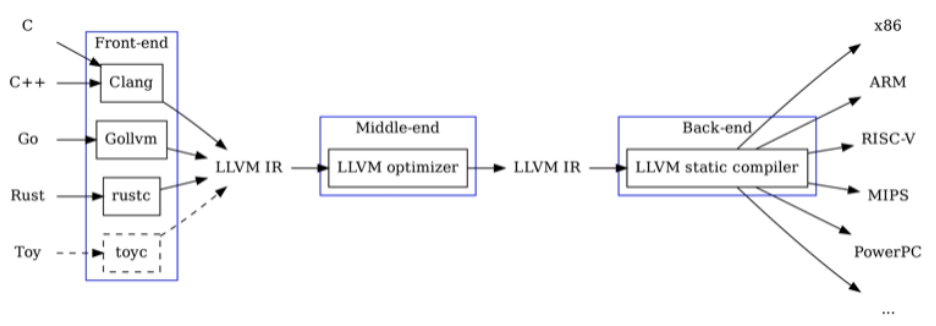
\includegraphics[width=10cm]{LLVMIR}
\end{figure}
为了更好的理解LLVM IR与汇编程序，下面将设计一个SysyY测试程序的LLVM IR与汇编代码，并链接SysY运行库,用LLVM/Clang、汇编器编译成成目标程序,验证运行结果是否正确 。

\subsection{测试程序}
先设计出测试程序的C源码，方便对照着编写LLVM IR和ARM汇编代码。
\lstset{
	columns=fixed,       
	numbers=left,                                        % 在左侧显示行号
	numberstyle=\tiny\color{gray},                       % 设定行号格式
	frame=none,                                          % 不显示背景边框
	backgroundcolor=\color[RGB]{245,245,244},            % 设定背景颜色
	keywordstyle=\color[RGB]{40,40,255},                 % 设定关键字颜色
	numberstyle=\footnotesize\color{darkgray},           
	commentstyle=\it\color[RGB]{0,96,96},                % 设置代码注释的格式
	stringstyle=\rmfamily\slshape\color[RGB]{128,0,0},   % 设置字符串格式
	showstringspaces=false,                              % 不显示字符串中的空格
	language=c,                                        % 设置语言
}
\begin{lstlisting}
	// SysY语言特性测试程序
	// 包含：数值运算、赋值、条件分支、循环、函数调用
	
	// 全局变量
	int global_var = 10;
	int array[5] = {1, 2, 3, 4, 5};
	
	// 数值运算函数
	int arithmetic_ops(int a, int b) {
		int sum = a + b;
		int diff = a - b;
		int prod = a * b;
		int quot = a / b;
		int mod = a % b;
		return sum + diff + prod + quot + mod;
	}
	
	// 条件分支函数
	int conditional_test(int x) {
		if (x > 0) {
			return 1;
		} else if (x < 0) {
			return -1;
		} else {
			return 0;
		}
	}
	
	// 循环函数 - while循环
	int while_loop(int n) {
		int sum = 0;
		int i = 1;
		while (i <= n) {
			sum = sum + i;
			i = i + 1;
		}
		return sum;
	}
	
	// 循环函数 - for循环
	int for_style_loop(int n) {
		int product = 1;
		int i;
		for (i = 1; i <= n; i = i + 1) {
			product = product * i;
		}
		return product;
	}
	
	// 递归函数
	int fibonacci(int n) {
		if (n <= 1) {
			return n;
		}
		return fibonacci(n - 1) + fibonacci(n - 2);
	}
	
	// 数组操作
	int array_sum() {
		int sum = 0;
		int i;
		for (i = 0; i < 5; i = i + 1) {
			sum = sum + array[i];
		}
		return sum;
	}
	
	int main() {
		int a, b, n;
		
		// 输入测试
		printf("Enter two integers: ");
		scanf("%d %d", &a, &b);
		
		// 数值运算测试
		printf("Arithmetic result: %d\n", arithmetic_ops(a, b));
		
		// 条件分支测试
		printf("Conditional test for %d: %d\n", a, conditional_test(a));
		printf("Conditional test for %d: %d\n", b, conditional_test(b));
		
		// 循环测试
		printf("Enter n for loop tests: ");
		scanf("%d", &n);
		
		printf("Sum 1 to %d (while): %d\n", n, while_loop(n));
		printf("Factorial of %d: %d\n", n, for_style_loop(n));
		
		// 递归测试
		if (n <= 10) {
			printf("Fibonacci(%d): %d\n", n, fibonacci(n));
		}
		
		// 数组测试
		printf("Array sum: %d\n", array_sum());
		
		// 全局变量测试
		printf("Global variable: %d\n", global_var);
		
		return 0;
	}
\end{lstlisting}

\subsection{LLVM IR编写}
首先明确，为了保证编写出的效果与SysY源代码等价，应该遵循以下编写原则：
\begin{itemize}
	\item 语义等价：相同输入产生相同输出
	\item 数据流等价：变量的生命周期和数据依赖关系一致
	\item 控制流等价：分支和循环的执行逻辑相同
	\item 函数调用等价：参数传递和返回值处理一致
\end{itemize}

那么，以数值运算函数为例，探究如何编写与之对应的正确的LLVM IR中间代码：

1.先对源代码进行简单的语义分析：

\begin{itemize}
	\item 识别变量和作用域
	
	可以明确：输入参数：a, b (int类型)；局部变量：sum, diff, prod, quot, mod (int类型)；返回值：int类型。
	\item 分析数据流
	
	a, b → sum = a + b
	
	a, b → diff = a - b  
	
	a, b → prod = a * b
	
	a, b → quot = a / b
	
	a, b → mod = a \% b
	
	sum, diff, prod, quot, mod → 返回值计算
	\item 分析控制流
	
	可以明确这部分代码：单一基本块，顺序执行
	；无分支，无循环
	；单一出口点(return)。
\end{itemize}

2.根据语义分析展开转换：

\begin{itemize}
	\item 函数签名转换
	
	例如  int arithmetic\_ops(int a, int b)
	
	转换为  define dso\_local i32 @arithmetic\_ops(i32 \%a, i32 \%b) \{
	
	转换规则：
	
	int → i32 (32位有符号整数)
	
	函数名前加@符号
	
	参数使用\%标记的SSA变量
	
	dso\_local表示符号在当前模块内
	\item 局部变量处理
	
	局部变量在LLVM IR中有两种处理方式：
	
	alloca指令（模拟栈分配）
	\lstset{
		columns=fixed,       
		numbers=left,                                        % 在左侧显示行号
		numberstyle=\tiny\color{gray},                       % 设定行号格式
		frame=none,                                          % 不显示背景边框
		backgroundcolor=\color[RGB]{245,245,244},            % 设定背景颜色
		keywordstyle=\color[RGB]{40,40,255},                 % 设定关键字颜色
		numberstyle=\footnotesize\color{darkgray},           
		commentstyle=\it\color[RGB]{0,96,96},                % 设置代码注释的格式
		stringstyle=\rmfamily\slshape\color[RGB]{128,0,0},   % 设置字符串格式
		showstringspaces=false,                              % 不显示字符串中的空格
		language=LLVM,                                        % 设置语言
	}
	\begin{lstlisting}
		entry:
			%sum = alloca i32, align 4
			%diff = alloca i32, align 4  
			%prod = alloca i32, align 4
			%quot = alloca i32, align 4
			%mod = alloca i32, align 4
	\end{lstlisting}
	
	和SSA形式
	\lstset{
		columns=fixed,       
		numbers=left,                                        % 在左侧显示行号
		numberstyle=\tiny\color{gray},                       % 设定行号格式
		frame=none,                                          % 不显示背景边框
		backgroundcolor=\color[RGB]{245,245,244},            % 设定背景颜色
		keywordstyle=\color[RGB]{40,40,255},                 % 设定关键字颜色
		numberstyle=\footnotesize\color{darkgray},           
		commentstyle=\it\color[RGB]{0,96,96},                % 设置代码注释的格式
		stringstyle=\rmfamily\slshape\color[RGB]{128,0,0},   % 设置字符串格式
		showstringspaces=false,                              % 不显示字符串中的空格
		language=LLVM,                                        % 设置语言
	}
	\begin{lstlisting}
		entry:
			%sum = add nsw i32 %a, %b
			%diff = sub nsw i32 %a, %b
			%prod = mul nsw i32 %a, %b
			%quot = sdiv i32 %a, %b
			%mod = srem i32 %a, %b
	\end{lstlisting}
	
	这里采用SSA形式：更接近编译器优化后的结果，还可以避免不必要的内存访问
	\item 算术运算转换
	
	见表2：
	\begin{table}[!htbp]
		\centering
		\begin{tabular}{ccccccccccc}
			\toprule  
			SysY运算& LLVM IR指令& 说明\\
			\midrule
			a + b& add nsw i32 \%a, \%b & nsw 即 no signed wrap\\
			a - b& sub nsw i32 \%a, \%b & 检测有符号溢出\\
			a * b& mul nsw i32 \%a, \%b & 有符号乘法\\
			a / b& sdiv i32 \%a, \%b & 有符号除法\\
			a \% b& srem i32 \%a, \%b & 有符号取余\\
			\bottomrule
		\end{tabular}
		\caption{算术转换}
		\label{table:t2}
	\end{table}
	\item 返回值计算
	\lstset{
		columns=fixed,       
		numbers=left,                                        % 在左侧显示行号
		numberstyle=\tiny\color{gray},                       % 设定行号格式
		frame=none,                                          % 不显示背景边框
		backgroundcolor=\color[RGB]{245,245,244},            % 设定背景颜色
		keywordstyle=\color[RGB]{40,40,255},                 % 设定关键字颜色
		numberstyle=\footnotesize\color{darkgray},           
		commentstyle=\it\color[RGB]{0,96,96},                % 设置代码注释的格式
		stringstyle=\rmfamily\slshape\color[RGB]{128,0,0},   % 设置字符串格式
		showstringspaces=false,                              % 不显示字符串中的空格
		language=c,                                        % 设置语言
	}
	\begin{lstlisting}
		return sum + diff + prod + quot + mod;
	\end{lstlisting}
	转换写成：
	\lstset{
		columns=fixed,       
		numbers=left,                                        % 在左侧显示行号
		numberstyle=\tiny\color{gray},                       % 设定行号格式
		frame=none,                                          % 不显示背景边框
		backgroundcolor=\color[RGB]{245,245,244},            % 设定背景颜色
		keywordstyle=\color[RGB]{40,40,255},                 % 设定关键字颜色
		numberstyle=\footnotesize\color{darkgray},           
		commentstyle=\it\color[RGB]{0,96,96},                % 设置代码注释的格式
		stringstyle=\rmfamily\slshape\color[RGB]{128,0,0},   % 设置字符串格式
		showstringspaces=false,                              % 不显示字符串中的空格
		language=LLVM,                                        % 设置语言
	}
	\begin{lstlisting}
		%temp1 = add nsw i32 %sum, %diff
		%temp2 = add nsw i32 %temp1, %prod  
		%temp3 = add nsw i32 %temp2, %quot
		%result = add nsw i32 %temp3, %mod
		ret i32 %result
	\end{lstlisting}
\end{itemize}

按照类似的过程，我们能逐步写出完整的LLVM IR代码：
\lstset{
	columns=fixed,       
	numbers=left,                                        % 在左侧显示行号
	numberstyle=\tiny\color{gray},                       % 设定行号格式
	frame=none,                                          % 不显示背景边框
	backgroundcolor=\color[RGB]{245,245,244},            % 设定背景颜色
	keywordstyle=\color[RGB]{40,40,255},                 % 设定关键字颜色
	numberstyle=\footnotesize\color{darkgray},           
	commentstyle=\it\color[RGB]{0,96,96},                % 设置代码注释的格式
	stringstyle=\rmfamily\slshape\color[RGB]{128,0,0},   % 设置字符串格式
	showstringspaces=false,                              % 不显示字符串中的空格
	language=LLVM,                                        % 设置语言
}
\begin{lstlisting}
	; SysY测试程序的LLVM IR实现
	target datalayout = "e-m:e-p270:32:32-p271:32:32-p272:64:64-i64:64-f80:128-n8:16:32:64-S128"
	target triple = "x86_64-pc-linux-gnu"
	
	; 声明SysY运行库函数
	declare i32 @getint()
	declare void @putint(i32)
	declare void @putch(i32)
	
	; 全局变量定义
	@global_var = dso_local global i32 10, align 4
	@array = dso_local global [5 x i32] [i32 1, i32 2, i32 3, i32 4, i32 5], align 16
	
	; 数值运算函数
	define dso_local i32 @arithmetic_ops(i32 %a, i32 %b) {
		entry:
		%sum = add nsw i32 %a, %b
		%diff = sub nsw i32 %a, %b
		%prod = mul nsw i32 %a, %b
		%quot = sdiv i32 %a, %b
		%mod = srem i32 %a, %b
		
		%temp1 = add nsw i32 %sum, %diff
		%temp2 = add nsw i32 %temp1, %prod
		%temp3 = add nsw i32 %temp2, %quot
		%result = add nsw i32 %temp3, %mod
		
		ret i32 %result
	}
	
	; 条件分支函数
	define dso_local i32 @conditional_test(i32 %x) {
		entry:
		%cmp_pos = icmp sgt i32 %x, 0
		br i1 %cmp_pos, label %if.positive, label %check_negative
		
		if.positive:
		ret i32 1
		
		check_negative:
		%cmp_neg = icmp slt i32 %x, 0
		br i1 %cmp_neg, label %if.negative, label %if.zero
		
		if.negative:
		ret i32 -1
		
		if.zero:
		ret i32 0
	}
	
	; while循环函数
	define dso_local i32 @while_loop(i32 %n) {
		entry:
		br label %while.cond
		
		while.cond:
		%sum.0 = phi i32 [ 0, %entry ], [ %sum.1, %while.body ]
		%i.0 = phi i32 [ 1, %entry ], [ %i.1, %while.body ]
		
		%cmp = icmp sle i32 %i.0, %n
		br i1 %cmp, label %while.body, label %while.end
		
		while.body:
		%sum.1 = add nsw i32 %sum.0, %i.0
		%i.1 = add nsw i32 %i.0, 1
		br label %while.cond
		
		while.end:
		ret i32 %sum.0
	}
	
	; 递归函数（斐波那契）
	define dso_local i32 @fibonacci(i32 %n) {
		entry:
		%cmp = icmp sle i32 %n, 1
		br i1 %cmp, label %base_case, label %recursive_case
		
		base_case:
		ret i32 %n
		
		recursive_case:
		%n_minus_1 = sub nsw i32 %n, 1
		%fib_n_1 = call i32 @fibonacci(i32 %n_minus_1)
		
		%n_minus_2 = sub nsw i32 %n, 2
		%fib_n_2 = call i32 @fibonacci(i32 %n_minus_2)
		
		%result = add nsw i32 %fib_n_1, %fib_n_2
		ret i32 %result
	}
	
	; 数组求和函数
	define dso_local i32 @array_sum() {
		entry:
		br label %for.cond
		
		for.cond:
		%sum.0 = phi i32 [ 0, %entry ], [ %sum.1, %for.body ]
		%i.0 = phi i32 [ 0, %entry ], [ %i.1, %for.body ]
		
		%cmp = icmp slt i32 %i.0, 5
		br i1 %cmp, label %for.body, label %for.end
		
		for.body:
		%arrayidx = getelementptr inbounds [5 x i32], [5 x i32]* @array, i64 0, i32 %i.0
		%load_val = load i32, i32* %arrayidx, align 4
		%sum.1 = add nsw i32 %sum.0, %load_val
		%i.1 = add nsw i32 %i.0, 1
		br label %for.cond
		
		for.end:
		ret i32 %sum.0
	}
	
	; 主函数
	define dso_local i32 @main() {
		entry:
		; 获取两个整数输入
		%a = call i32 @getint()
		%b = call i32 @getint()
		
		; 数值运算测试
		%arith_result = call i32 @arithmetic_ops(i32 %a, i32 %b)
		call void @putint(i32 %arith_result)
		call void @putch(i32 10)  ; 换行符
		
		; 条件分支测试
		%cond_a = call i32 @conditional_test(i32 %a)
		call void @putint(i32 %cond_a)
		call void @putch(i32 10)
		
		%cond_b = call i32 @conditional_test(i32 %b)
		call void @putint(i32 %cond_b)
		call void @putch(i32 10)
		
		; 循环测试
		%n = call i32 @getint()
		
		%while_result = call i32 @while_loop(i32 %n)
		call void @putint(i32 %while_result)
		call void @putch(i32 10)
		
		; 递归测试（限制输入范围）
		%small_check = icmp sle i32 %n, 10
		br i1 %small_check, label %do_fibonacci, label %skip_fibonacci
		
		do_fibonacci:
		%fib_result = call i32 @fibonacci(i32 %n)
		call void @putint(i32 %fib_result)
		call void @putch(i32 10)
		br label %array_test
		
		skip_fibonacci:
		br label %array_test
		
		array_test:
		; 数组测试
		%array_result = call i32 @array_sum()
		call void @putint(i32 %array_result)
		call void @putch(i32 10)
		
		; 全局变量测试
		%global_val = load i32, i32* @global_var, align 4
		call void @putint(i32 %global_val)
		call void @putch(i32 10)
		
		ret i32 0
	}
\end{lstlisting}

编译并测试成功，如下图所示

\begin{figure}[H]
	\centering	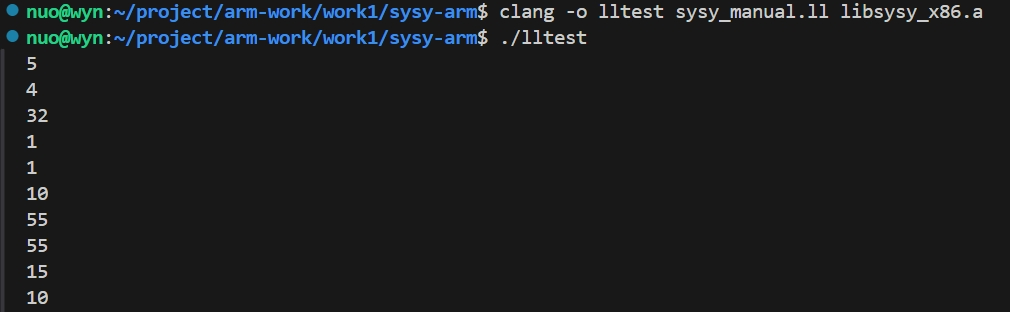
\includegraphics[width=10cm]{llvmtest}
\end{figure}

\subsection{ARM汇编编写}
要编写与源代码等价的、能正确运行的汇编代码，应满足以下要求：

\begin{itemize}
	\item 语义等价性：ARM汇编完全保持了C语言的执行语义
	\item 控制流映射：while循环被转换为条件分支+跳转的组合
	\item 数据流保持：变量的生命周期和数据依赖关系得到正确维护
	\item 调用约定遵循：正确使用ARM 约定进行参数传递和返回值处理
\end{itemize}

接下来以循环函数while\_loop的汇编编写为例探究汇编代码的编写：

1.先对这段程序进行简单的语义分析：

\begin{itemize}
	\item 输入: 整数n
	\item 输出: 1+2+3+...+n的和
	\item 算法流程:
	
	初始化sum=0, i=1
	
	检查条件i <= n
	
	如果条件成立：sum += i, i++, 跳转到步骤2
	
	如果条件不成立：返回sum
\end{itemize}

2.ARM汇编逐步转换：
\paragraph{函数框架设计}
\lstset{
	columns=fixed,       
	numbers=left,                                        % 在左侧显示行号
	numberstyle=\tiny\color{gray},                       % 设定行号格式
	frame=none,                                          % 不显示背景边框
	backgroundcolor=\color[RGB]{245,245,244},            % 设定背景颜色
	keywordstyle=\color[RGB]{40,40,255},                 % 设定关键字颜色
	numberstyle=\footnotesize\color{darkgray},           
	commentstyle=\it\color[RGB]{0,96,96},                % 设置代码注释的格式
	stringstyle=\rmfamily\slshape\color[RGB]{128,0,0},   % 设置字符串格式
	showstringspaces=false,                              % 不显示字符串中的空格
	language=c,                                        % 设置语言
}
\begin{lstlisting}
	.align 2
	.global while_loop
	.type while_loop, %function
	while_loop:
	// 函数入口 - w0包含参数n
	// 需要决定：用寄存器还是栈来存储局部变量？
	// 这个简单函数可以全部用寄存器
	
	// 返回值通过w0寄存器返回
	ret
\end{lstlisting}
接着确定寄存器分配：

w0: 输入参数n，后续用作返回值

w1: sum变量

w2: i变量
\paragraph{循环条件检查}
\lstset{
	columns=fixed,       
	numbers=left,                                        % 在左侧显示行号
	numberstyle=\tiny\color{gray},                       % 设定行号格式
	frame=none,                                          % 不显示背景边框
	backgroundcolor=\color[RGB]{245,245,244},            % 设定背景颜色
	keywordstyle=\color[RGB]{40,40,255},                 % 设定关键字颜色
	numberstyle=\footnotesize\color{darkgray},           
	commentstyle=\it\color[RGB]{0,96,96},                % 设置代码注释的格式
	stringstyle=\rmfamily\slshape\color[RGB]{128,0,0},   % 设置字符串格式
	showstringspaces=false,                              % 不显示字符串中的空格
	language=c,                                        % 设置语言
}
\begin{lstlisting}
	.L_while_cond:
		cmp w2, w0              // compare i with n
		bgt .L_while_end        // if i > n, exit
	    //后面是循环体
\end{lstlisting}
cmp w2, w0 执行 w2-w0 并设置条件标志

bgt 检查有符号比较结果，如果i > n执行跳转

否则顺序执行到循环体
\paragraph{循环体实现}
\lstset{
	columns=fixed,       
	numbers=left,                                        % 在左侧显示行号
	numberstyle=\tiny\color{gray},                       % 设定行号格式
	frame=none,                                          % 不显示背景边框
	backgroundcolor=\color[RGB]{245,245,244},            % 设定背景颜色
	keywordstyle=\color[RGB]{40,40,255},                 % 设定关键字颜色
	numberstyle=\footnotesize\color{darkgray},           
	commentstyle=\it\color[RGB]{0,96,96},                % 设置代码注释的格式
	stringstyle=\rmfamily\slshape\color[RGB]{128,0,0},   % 设置字符串格式
	showstringspaces=false,                              % 不显示字符串中的空格
	language=c,                                        % 设置语言
}
\begin{lstlisting}
		add w1, w1, w2          // sum += i
		add w2, w2, #1          // i++
		b .L_while_cond
\end{lstlisting}
add w1, w1, w2: 目标寄存器w1 = w1 + w2

add w2, w2, \#1: i自增1，立即数加法

b .L\_while\_cond: 无条件跳转回条件检查

\paragraph{循环结束和返回}
\lstset{
	columns=fixed,       
	numbers=left,                                        % 在左侧显示行号
	numberstyle=\tiny\color{gray},                       % 设定行号格式
	frame=none,                                          % 不显示背景边框
	backgroundcolor=\color[RGB]{245,245,244},            % 设定背景颜色
	keywordstyle=\color[RGB]{40,40,255},                 % 设定关键字颜色
	numberstyle=\footnotesize\color{darkgray},           
	commentstyle=\it\color[RGB]{0,96,96},                % 设置代码注释的格式
	stringstyle=\rmfamily\slshape\color[RGB]{128,0,0},   % 设置字符串格式
	showstringspaces=false,                              % 不显示字符串中的空格
	language=c,                                        % 设置语言
}
\begin{lstlisting}
	.L_while_end:
		mov w0, w1              // return sum
		ret
\end{lstlisting}
返回值约定:w0用于返回32位整数

需要将结果从w1移动到w0
\paragraph{完整ARM汇编实现}
\lstset{
	columns=fixed,       
	numbers=left,                                        % 在左侧显示行号
	numberstyle=\tiny\color{gray},                       % 设定行号格式
	frame=none,                                          % 不显示背景边框
	backgroundcolor=\color[RGB]{245,245,244},            % 设定背景颜色
	keywordstyle=\color[RGB]{40,40,255},                 % 设定关键字颜色
	numberstyle=\footnotesize\color{darkgray},           
	commentstyle=\it\color[RGB]{0,96,96},                % 设置代码注释的格式
	stringstyle=\rmfamily\slshape\color[RGB]{128,0,0},   % 设置字符串格式
	showstringspaces=false,                              % 不显示字符串中的空格
	language=c,                                        % 设置语言
}
\begin{lstlisting}
	.arch armv8-a
	.text
	
	// SysY运行库函数声明
	.extern getint
	.extern putint
	.extern putch
	
	// 全局变量定义
	.section .data
	.align 2
	.global global_var
	global_var:
		.word 10
	
	.global array
	array:
		.word 1, 2, 3, 4, 5
	
	.text
	
	// 数值运算函数
	.align 2
	.global arithmetic_ops
	.type arithmetic_ops, %function
	arithmetic_ops:
		// w0 = a, w1 = b
		add w2, w0, w1          // sum = a + b
		sub w3, w0, w1          // diff = a - b
		mul w4, w0, w1          // prod = a * b
		sdiv w5, w0, w1         // quot = a / b
		msub w6, w5, w1, w0     // mod = a - (quot * b)
	
		add w7, w2, w3          // temp1 = sum + diff
		add w7, w7, w4          // temp2 = temp1 + prod
		add w7, w7, w5          // temp3 = temp2 + quot
		add w0, w7, w6          // result = temp3 + mod
	
		ret
	
	// 条件分支函数
	.align 2
	.global conditional_test
	.type conditional_test, %function
	conditional_test:
		cmp w0, #0
		bgt .L_positive
		blt .L_negative
	
	.L_zero:
		mov w0, #0
		ret
	
	.L_positive:
		mov w0, #1
		ret
	
	.L_negative:
		mov w0, #-1
		ret
	
	// while循环函数
	.align 2
	.global while_loop
	.type while_loop, %function
	while_loop:
		mov w1, #0              // sum = 0
		mov w2, #1              // i = 1
	
	.L_while_cond:
		cmp w2, w0              // compare i with n
		bgt .L_while_end        // if i > n, exit
	
		add w1, w1, w2          // sum += i
		add w2, w2, #1          // i++
		b .L_while_cond
	
	.L_while_end:
		mov w0, w1              // return sum
		ret
	
	// 递归函数（斐波那契）
	.align 2
	.global fibonacci
	.type fibonacci, %function
	fibonacci:
		stp x29, x30, [sp, #-32]!
		mov x29, sp
		str w0, [sp, #28]       // 保存n
	
		cmp w0, #1
		ble .L_fib_base
	
		sub w0, w0, #1          // n-1
		bl fibonacci            // fib(n-1)
		str w0, [sp, #24]       // 保存fib(n-1)
	
		ldr w0, [sp, #28]       // 加载n
		sub w0, w0, #2          // n-2
		bl fibonacci            // fib(n-2)
	
		ldr w1, [sp, #24]       // 加载fib(n-1)
		add w0, w0, w1          // fib(n-1) + fib(n-2)
		b .L_fib_end
	
	.L_fib_base:
		ldr w0, [sp, #28]       // 返回n (0或1)
		
	.L_fib_end:
		ldp x29, x30, [sp], #32
		ret
	
	// 数组求和函数
	.align 2
	.global array_sum
	.type array_sum, %function
	array_sum:
		adrp x1, array          // 获取数组地址
		add x1, x1, :lo12:array
	
		mov w0, #0              // sum = 0
		mov w2, #0              // i = 0
		
	.L_array_loop:
		cmp w2, #5              // compare i with 5
		bge .L_array_end        // if i >= 5, exit
	
		ldr w3, [x1, w2, uxtw #2]  // 加载array[i]
		add w0, w0, w3          // sum += array[i]
		add w2, w2, #1          // i++
		b .L_array_loop
	
	.L_array_end:
		ret
	
	// 主函数
	.align 2
	.global main
	.type main, %function
	main:
		stp x29, x30, [sp, #-48]!
		mov x29, sp
	
		// 获取输入a, b
		bl getint
		str w0, [sp, #20]       // 保存a
	
		bl getint
		str w0, [sp, #24]       // 保存b
	
		// 数值运算测试
		ldr w0, [sp, #20]       // 加载a
		ldr w1, [sp, #24]       // 加载b
		bl arithmetic_ops
		bl putint
		mov w0, #10
		bl putch               // 换行
	
		// 条件分支测试
		ldr w0, [sp, #20]       // 加载a
		bl conditional_test
		bl putint
		mov w0, #10
		bl putch
	
		ldr w0, [sp, #24]       // 加载b
		bl conditional_test
		bl putint
		mov w0, #10
		bl putch
	
		// 获取n用于循环测试
		bl getint
		str w0, [sp, #28]       // 保存n
	
		// while循环测试
		ldr w0, [sp, #28]
		bl while_loop
		bl putint
		mov w0, #10
		bl putch
	
		// 递归测试（限制范围）
		ldr w0, [sp, #28]
		cmp w0, #10
		bgt .L_skip_fib
	
		bl fibonacci
		bl putint
		mov w0, #10
		bl putch
	
		.L_skip_fib:
			// 数组测试
			bl array_sum
			bl putint
			mov w0, #10
			bl putch
	
	// 全局变量测试
		adrp x0, global_var
		add x0, x0, :lo12:global_var
		ldr w0, [x0]
		bl putint
		mov w0, #10
		bl putch
		
		mov w0, #0
		ldp x29, x30, [sp], #48
		ret
\end{lstlisting}

编译并测试成功，如下图所示

\begin{figure}[H]
	\centering	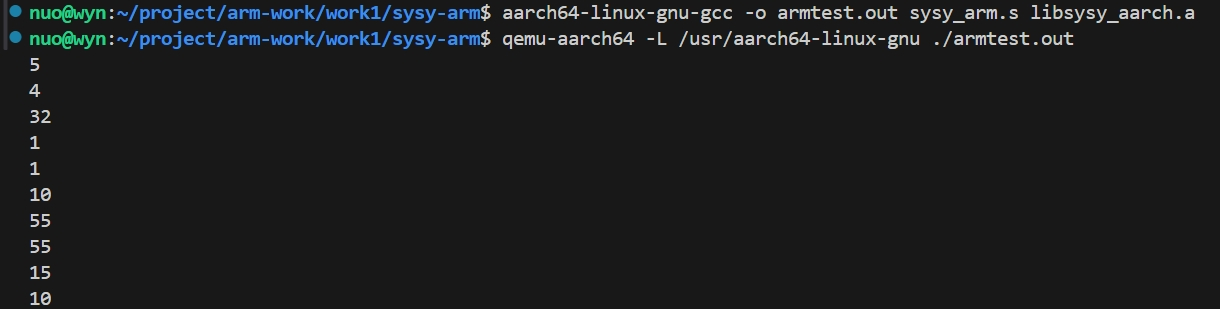
\includegraphics[width=10cm]{armtest}
\end{figure}

\section{结论}
本实验通过对编译工具链的深入研究和实践操作,系统地掌握了从源代码到可执行程序的完整转换过程。主要完成了以下工作和认识:

1.编译流程的深入理解: 通过对阶乘程序的逐步分析,清晰地观察到预处理器如何展开宏定义和头文件、编译器如何进行词法语法分析并生成抽象语法树、如何转换为LLVM IR中间表示、如何生成目标平台的汇编代码,以及汇编器和链接器如何协同工作最终生成可执行文件。每个阶段的输出都得到了详细分析,加深了对编译原理的理解。

2.LLVM IR编程实践: 成功设计并实现了包含SysY语言核心特性的LLVM IR程序,涵盖了算术运算、条件分支、while循环、递归、数组操作等语言特性。通过手工编写IR代码,深刻理解了SSA形式、基本块、phi节点等中间表示的核心概念,以及LLVM如何通过平台无关的中间表示实现前后端分离。

3.ARM汇编编程实践: 完成了与源程序语义等价的ARM汇编代码编写,正确实现了寄存器分配、栈帧管理、函数调用约定、控制流转换等底层细节。通过汇编编程,理解了高级语言特性如何映射到机器指令层面,以及调用约定、栈保护等运行时机制的实现。

4.理论与实践的结合: 实验不仅验证了理论知识,更通过实际操作加深了理解。手工编写的LLVM IR和ARM汇编程序均能成功链接SysY运行库并正确执行,证明了对编译原理核心概念的准确把握。

通过本次实验,不仅掌握了编译器的工作原理和实现技术,更培养了系统思维和工程实践能力,为后续的编译器设计与实现课程打下了坚实基础。

\end{document}
